%%%%%%%%%%%%%%%%%%%%%%%%%%%%%%%%%%%%%%%%%%%%%%%%%%%%%%%%%%%%%%%%%%%%%%%%%%%%%%%%
%\documentclass[12pt,papel,twoside]{ibtesis}
% \documentclass[12pt]{ibtesis}

% \documentclass[11pt,papel,oneside,singlespace]{ibtesis}
\documentclass[12pt,papel,oneside]{ibtesis}
% \documentclass[12pt,papel,preprint,singlespace,oneside]{ibtesis}
\decimalpoint
%%%%%%%%%%%%%%%%%%%%% Paquetes extra %%%%%%%%%%%%%%%%%%%%%%%%%%%%%%%%%%%%%%%%%%%
% Por conveniencia: aqu\'{\i} puede cargar todos los paquetes y definir los comandos 
% que necesite
\usepackage{ibextra}
\usepackage[utf8]{inputenc}
\usepackage{subcaption}  % Enable figure captions or figure notes
\usepackage{float}
\usepackage{nicefrac}
\usepackage{mathtools}
\usepackage{textcomp}

\usepackage{multirow}
\usepackage{amsfonts}

\usepackage{hyperref}
\usepackage{tablefootnote}

\usepackage{scalerel}
\usepackage{physics}


\usepackage{xparse}
\let\realItem\item % save a copy of the original item
\makeatletter
\NewDocumentCommand\myItem{ o }{%
   \IfNoValueTF{#1}%
      {\realItem}% add an item
      {\realItem[#1]\def\@currentlabel{#1}}% add an item and update label
}
\makeatother

\usepackage{enumitem}    
\setlist[enumerate]{
    before=\let\item\myItem%,       % use \myItem in enumerate
    %label=\textnormal{(\arabic*)}, % format the label
    %widest=(2')                    % set the widest label
}

%%%%%%%%%%%%%%%%%%%%%%%%%%%%%%%%%%%%%%%%%%%%%%%%%%%%%%%%%%%%%%%%%%%%%%%%%%%%%%%%
%%%%%%%%%%%%%%%%%%%%% Informacion sobre la tesis %%%%%%%%%%%%%%%%%%%%%%%%%%%%%%%
\title{Análisis de las direcciones de arribo de rayos cósmicos de ultra-alta energía en el Observatorio Pierre Auger}
\author{Evelyn~G.~Coronel}
\director{Dra.~Silvia Mollerach}
%\codirector{Dr.~J.~Otro m\'{a}s}b
\carrera{Tesis de Maestría en Ciencias F\'{\i}sicas}
\grado{Maestrando}
\laboratorio{Partículas y Campos -- Centro At\'{o}mico Bariloche}
\jurado{Dr.~Diego~Harari (Instituto Balseiro)}

\palabrasclave{Rayos Cósmicos, Análisis de datos, Instituto Balseiro}
%\keywords{Cosmic Rays, Data Analysis, Balseiro Institute}
%\neembaeguasu{Mba'e michĩ yvágagui ouva, Mbo'ehaoguasu Balseiro}
% Si queremos poner la fecha manualmente:
% \date{Diciembre de 2099}

%%%%%%%%%%%%%%%%%%%%%%%%%%%%%%%%%%%%%%%%%%%%%%%%%%%%%%%%%%%%%%%%%%%%%%%%%%%%%%%%
\titlepagefalse % Si no quiere compilar la portada descomente esta linea
%\includeonly{apendices} % Compilar s\'{o}lo estos archivos 
%\graphicspath{{/h}} % Lugar donde encontrar las figuras generales (se puede poner uno en cada cap{\'{\i}}tulo)
%%%%%%%%%%%%%%%%%%%%%%%%%%%%%%%%%%%%%%%%%%%%%%%%%%%%%%%%%%%%%%%%%%%%%%%%%%%%%%%%


\setcounter{tocdepth}{6}
\setcounter{secnumdepth}{6}
\begin{document}


\chapter{Método East-West}

El método de Rayleigh se basa ajustar el flujo de CRs en función de la ascensión recta mediante una función armónica. El mismo permite calcular la amplitud de la anisotropía para distintos armónicos, su fase y la probabilidad de detectar la misma señal debido a fluctuaciones de una distribución isótropa de RCs. 

La dificultad en utilizar el método Rayleigh recae en procesamiento de los datos: efectos del clima,  variaciones en el área del Observatorio, y la sensibilidad de los instrumentos deben tenerse en cuenta.  Los efectos mencionados deben ser corregidos de la señal medida de los eventos, ya que los mismos inducen modulaciones espurias en el análisis.

En el método East - West consiste en el ajuste de una función armónica a la diferencia entre los flujos de eventos provenientes del Este y del Oeste. Si se consideran que las modulaciones espurias producidas por los efectos atmosféricos y sistemáticos son las mismas en ambas direcciones, la diferencia de flujos remueve estos efectos sin realizar correcciones adicionales. Una desventaja de este método es que su sensibilidad es menor que el método de Rayleigh \cite{taborda}.


\section{Descripción de una anisotropía dipolar}
Las anisotropías en las direcciones de llegada de los RCs indican que ciertas zonas del cielo tienen una variación significativa con respecto a la media de flujo de RCs. Esta anisotropía puede describirse mediante funciones armónicas, la más sencilla es la anisotropía dipolar es una aproximación a primer orden.

Una anisotropía dipolar se puede describir de la siguiente forma:
\begin{equation}
    \Phi(\hat{\bf{u}}) = \Phi_0(1+\bf{d}\cdot\hat{\bf{u}})
    \label{eq:dipolo_general}
\end{equation}
\noindent donde $\Phi_0$ es el flujo medio de eventos, $\hat{\bf{u}}$ es un versor que apunta a la dirección a estudiar, y $\bf{d}$ es el vector con módulo igual a la amplitud del dipolo y con dirección al eje del mismo. Tomando coordenadas ecuatoriales \footnote{Referencia al apéndice de ecuatoriales}, la dirección de $\bf{d}$ es $(\alpha_d, \delta_d$) y  de $\hat{\bf{u}}$ es $(\alpha, \delta)$, por lo tanto  el producto escalar  entre estos vectores se puede escribir de la siguiente manera \footnote{Falta mencionar el producto de versor de esta representación para decir sale de acá. Eso va a estar en el apéndice porque el cálculo me  sale fácil poniendo  todo en cartesianas.)}:
\begin{equation}
    \textbf{d}\cdot\hat{\bf{u}}= d (\cos\delta_d \cos\delta \cos(\alpha - \alpha_d) + \sin\delta_d  \sin\delta)
    \label{eq:product_ud}
\end{equation}


Otro aspecto importante de la representación del dipolo en coordenadas ecuatoriales, es que la proyección de la amplitud del dipolo sobre el plano ecuatorial se puede aproximar de la siguiente manera:
\begin{equation}
    r_1 \simeq d_\perp \langle \cos\delta \rangle
    \label{eq:fourier_perp}
\end{equation}
donde $r_1$ es la amplitud de la aproximación a primer orden en Fourier, y $\langle \cos\delta \rangle$ es el valor medio de $\cos\delta $ de los eventos utilizados para realizar la aproximación mencionada.

\subsection{Representación en coordenadas locales de la anisotropía dipolar}
Podemos reescribir el producto escalar entre dipolo $\textbf{d}$ y el versor $\hat{u}$ apunta en la dirección cualquiera mediante las coordenadas locales $\theta$ y $\phi$ \footnote{Referencia locales apéndice}.
\begin{align}
    \textbf{d} &=  d_x(\alpha^0)\hat{x} +  d_y(\alpha^0)\hat{y}+ d_z(\alpha^0)\hat{z} \\
    \hat{\bf{u}} &=\sin\theta \cos\phi \hat{x} + \sin\theta \sin\phi \hat{y} + \cos\theta\hat{z}\\
    \textbf{d}\cdot\hat{\bf{u}} &= d_x(\alpha^0)\sin\theta \cos\phi
    + d_y(\alpha^0) \sin\theta \sin\phi  
     + d_z(\alpha^0)\cos\theta \label{eq:dot-prod-local}
\end{align}
donde los versores $\hat{x}$, $\hat{y}$ y $\hat{z}$ apuntan a la dirección Este, Norte  y  del cenit respectivamente. 

El dipolo está fijo en el cielo pero visto desde las coordenadas locales para poder trabajar con $\theta$ y $\phi$, sus proyecciones  proyecciones $d_x$, $d_y$ y $d_z$  tienen una dependencia con la ascensión recta  $\alpha^0$ y declinación $\delta_0$ del cenit. 

\section{Descripción formal del método East-West}

    \subsection{Flujo de eventos del Este y Oeste}
    El flujo de eventos observado $I^{obs}(\alpha^0)$ para la ascensión recta del cenit $\alpha^0$ entre los ángulos azimutales $\phi_1$ y $\phi_2$ puede calcularse mediante el flujo total de RCs $\Phi(\theta, \phi, \alpha^0)$ (expresado en coordenadas locales) como
    \begin{equation}
        I^{obs}(\alpha^0) = \int_{\phi_1}^{\phi_2} d\phi \int_{0}^{\theta_{max}} d\theta \sin\theta \tilde{\omega}(\theta, \alpha^0) \Phi(\theta, \phi, \alpha^0),
        \label{eq:rate_general}
    \end{equation}
    \noindent  donde  el término $\tilde{\omega}(\theta, \alpha^0)$ representa la exposición del Observatorio. Este término también incluye los efectos sistemáticos y atmosféricos, como la variación de los hexágonos del arreglo y las correcciones de la modulación del clima, mediante  su dependencia con $\alpha^0$.

    Para calcular los flujos de eventos del Este y Oeste, $I^{obs}_E$ y $I_O^{obs}$ respectivamente, se integra la Ec.\ref{eq:rate_general} en los siguientes  rangos: para el Este: entre $\phi_1=\nicefrac{-\pi}{2}$ y $\phi_2=\nicefrac{\pi}{2}$ y para el Oeste: entre $\phi_1=\nicefrac{\pi}{2}$ y $\phi_2=\nicefrac{3\pi}{2}$.

    \subsection{Aproximaciones del método}
    Se considera que pueden  desacoplarse de las variables $\theta$ y $\alpha^0$, por lo tanto, podemos expresar $\tilde{\omega}$ de la siguiente manera:
    \begin{equation}
        \tilde{\omega}(\theta, \alpha^0) = \omega(\theta)F(\alpha^0)
    \end{equation}    
    
    A su vez, consideremos que las amplitudes de las variaciones asociadas a $\tilde{\omega}$ son pequeñas con respecto al valor medio, por lo que se puede tomar la expansión en primer orden de la función $F(\alpha^0)$:
    \begin{equation}
        \tilde{\omega}(\theta, \alpha^0) = \omega(\theta)\big(1 + \eta(\alpha^0) \big)
        \label{eq:omega_expandido}
    \end{equation}
    \subsection{Cálculo de la diferencia de flujos}
  
    Teniendo en cuenta la Ec.\ref{eq:omega_expandido} y \ref{eq:dipolo_general}, se tiene la siguiente expresión:
    \begin{align}
        I^{obs}(\alpha^0) &= \int_{\phi_1}^{\phi_2} d\phi \int_{0}^{\theta_{max}} d\theta  \sin\theta \omega(\theta)\big(1 + \eta(\alpha^0) \big) \Phi_0 ( 1 +  \textbf{d}\cdot\hat{\bf{u}}) \label{eq:I-obs}
    \end{align}
    donde la primera parte  de la igualdad  puede simplificarse con una definición apropiada  \footnote{ $
        \text{Por simplicidad, definimos la siguiente expresión: }
      \overline{f(\theta)} = \int_{0}^{\theta_{max}} d\theta \sin\theta \omega(\theta) f(\theta)
      \label{eq:media_angular}
  $
  \noindent, donde $\overline{f(\theta)}$ es la media de la función $f(\theta)$ sobre el ángulo cenital pesado por la exposición del Observatorio $\omega(\theta)$, hasta  un ángulo máximo de $\theta_{max}$. En este trabajo se centra en eventos hasta 2 EeV, por lo que $\theta_{max}=60^o$ para los datos del Observatorio.}. Además dado que la integral sobre $\phi$ tiene el mismo valor para el Este y Oeste, se  obtiene que la primera parte se puede escribir de la siguiente forma
    \begin{align*}
        &\int_{\phi_1}^{\phi_2} d\phi \int_{0}^{\theta_{max}} d\theta \sin\theta \omega(\theta)\big(1 + \eta(\alpha^0) \big) \Phi_0 
        = \Phi_0 (1+ \eta(\alpha^0)) \overline{1}. 
    \end{align*}
    Trabajando con la segunda parte de la expresión \ref{eq:I-obs}, si  consideramos la expresión \ref{eq:dot-prod-local} del producto escalar $\textbf{d}\cdot\hat{\bf{u}}$ en coordenadas locales, e integramos el ángulo  $\phi$ entre $[\nicefrac{-\pi}{2}, \nicefrac{\pi}{2}]$ o $[\nicefrac{\pi}{2}, \nicefrac{3\pi}{2}]$, se obtiene que:

    \begin{align}
        &\int_{\phi_1}^{\phi_2} d\phi \int_{0}^{\theta_{max}} d\theta \sin\theta \omega(\theta)\big(1 + \eta(\alpha^0) \big) \Phi_0 \textbf{d}\cdot\hat{\bf{u}}=\\
        &=\Phi_0 (1+ \eta(\alpha^0)) \int_{0}^{\theta_{max}}  d\theta (\pm 2d_x(\alpha^0)\sin\theta 
        + \pi d_z(\alpha^0)\cos\theta) \label{segundo_term}
    \end{align}
    \noindent donde $+2$ corresponde al Este y $-2$ al Oeste. No hay una dependencia con la proyección del dipolo $d_y$ porque en la integral aparece el término $\int_{\phi_1}^{\phi_2}\, d\phi\, d_y(\alpha^0) \sin\theta \sin\phi $, que se anula al integrar sobre el Este y Oeste.


    %  Al integrar el ángulo  $\phi$ entre $[\nicefrac{-\pi}{2}, \nicefrac{\pi}{2}]$ o $[\nicefrac{\pi}{2}, \nicefrac{3\pi}{2}]$, el segundo término  se anula, por lo que la expresión \ref{segundo_term} queda como:
    % \begin{align*}
    %     &\int_{\phi_1}^{\phi_2} d\phi \int_{0}^{\theta_{max}}  d\theta \sin\theta \omega(\theta)\textbf{d}\cdot\hat{\bf{u}} =\\
    %     &\int_{0}^{\theta_{max}}  d\theta (\pm 2d_x(\alpha^0)\sin\theta 
    %     + \pi d_z(\alpha^0)\cos\theta)
    % \end{align*}     
    % \noindent donde $+2$ corresponde al Este y $-2$ al Oeste. 
    
     Usando la definición dada en la nota \ref{eq:media_angular} y la expresión \ref{segundo_term}, podemos reescribir la expresión \ref{eq:I-obs} y los flujos para el Este y el Oeste como:
    \begin{align*}
    I^{obs}_E&= \Phi_0 (1+ \eta(\alpha^0)) \Big( \pi\overline{1} + 2d_x(\alpha^0)\overline{\sin\theta} + \pi d_z(\alpha^0)\overline{\cos\theta}  \Big) \\
        I^{obs}_O&= \Phi_0 (1+ \eta(\alpha^0)) \Big( \pi \overline{1} - 2d_x(\alpha^0)\overline{\sin\theta}   + \pi d_z(\alpha^0)\overline{\cos\theta} \Big) \\
        I^{obs}&= \Phi_0 (1+ \eta(\alpha^0)) \Big( 2\pi\overline{1} +\pi d_z(\alpha^0)\overline{\cos\theta}  \Big)
    \end{align*}
    Ya que se busca calcular la diferencia entre los flujos provenientes del Este y del Oeste, $I^{obs}_E $ y $  I^{obs}_O $ respectivamente, esta resta queda como:
    \begin{equation*}
        I^{obs}_E -  I^{obs}_O = 4 \Phi_0 (1+ \eta(\alpha^0)) \,  d_x(\alpha^0)\overline{\sin\theta}
    \end{equation*}

    Para obtener las componentes del vector $\bf{d}$, tenemos que considerar que las mismas están en el plano x-z. Para hacer esto, consideremos a los versores $\hat{\bf{u}}_x$ y $\hat{\bf{u}}_z$ que apuntan al cenit y al Este respectivamente. Podemos obtener las proyecciones con un producto escalar con los versores en las direcciones de interés:
    \begin{equation}
        d_x(\alpha^0) \hat{x} =  (\textbf{d}\cdot\hat{\bf{u}}_x)\hat{\bf{u}}_x \rightarrow d_x(\alpha^0) = \textbf{d}\cdot\hat{\bf{u}}_x,
    \end{equation}
    donde estos versores en coordenadas ecuatoriales se escriben como:
    $\hat{\bf{u}}_z = (\alpha^0,\delta_0 )$ y $ \hat{\bf{u}}_x = (\alpha^0 + \frac{\pi}{2},0)$ \footnote{Se suma  $\frac{\pi}{2}$ para apuntar al Este, cuando el versor recorre $\nicefrac{\pi}{2}$ en ascensión recta, llega al plano del ecuador que tiene declinación $0$.}.

    % \item 
   
    % Volviendo a la expresión de $I^{obs}$, teniendo en cuenta que necesitamos  $I^{obs}_E$ y $I^{obs}_O$:
    % \begin{align*}
    %     I^{obs}_E&= \Phi_0 (1+ \eta(\alpha^0)) \Big( \pi\overline{1} + 2d_x(\alpha^0)\overline{\sin\theta} + \pi d_z(\alpha^0)\overline{\cos\theta}  \Big) \\
    %     I^{obs}_O&= \Phi_0 (1+ \eta(\alpha^0)) \Big( \pi \overline{1} - 2d_x(\alpha^0)\overline{\sin\theta}   + \pi d_z(\alpha^0)\overline{\cos\theta} \Big) 
    % \end{align*}

    % \item 
    
    % \item 
    Usando la expresión \ref{eq:product_ud} para el producto escalar en coordenadas ecuatoriales, se obtienen las componentes:
    \begin{align*}
        d_z=\textbf{d}\cdot\hat{\bf{u}}_z &= d (\cos\delta_d \cos\delta_0 \cos(\alpha^0 - \alpha_d) + \sin\delta_d  \sin\delta_0)\\
        d_x=\textbf{d}\cdot\hat{\bf{u}}_x &= d (\cos\delta_d \cos(\alpha^0 +\frac{\pi}{2} - \alpha_d) 
        = -d\cos\delta_d \sin(\alpha^0  - \alpha_d)
    \end{align*}
    
     Entonces la diferencia entre flujos queda como:
    \begin{equation}
        I^{obs}_E -  I^{obs}_O =-4d \Phi_0 (1+ \eta(\alpha^0)) \cos\delta_d \sin(\alpha^0  - \alpha_d)\overline{\sin\theta}
        \label{resta}
    \end{equation}

    Esta diferencia se debe relacionar con la variación del flujo verdadero $I(\alpha^0)$, es decir el flujo que se observaría si no existieran variaciones temporales en ascensión recta en la exposición, que implicaría $\eta(\alpha^0)=0$. 

    La variación del flujo verdadero en ascensión recta provee información sobre la componente $d_z$ del dipolo. 
    \begin{align}
        \dv{I(\alpha^0)}{\alpha^0}  & = 2\pi\Phi_0 \overline{\cos\theta} \dv{\,d_z(\alpha^0) }{\alpha^0}\\ 
        \dv{I(\alpha^0)}{\alpha^0} &= -2d\pi\Phi_0 \overline{\cos\theta}\cos\delta_d \cos\delta_0 \sin(\alpha^0 - \alpha_d) \label{total_flux}
    \end{align}

    Para llegar a la expresión \ref{resta}, hicimos la expansión hasta el primer orden de $\tilde{\omega}(\theta, \alpha^0)$ y de $\bf\Phi(\alpha, \delta)$, por lo tanto, para ser consistentes en el orden de aproximación, se desprecia el término de segundo orden de la expresión \ref{resta} que es proporcional de $\eta \cdot d$ y la expresión \ref{resta} queda:
        \begin{equation}
            I^{obs}_E -  I^{obs}_O \approx -4d \Phi_0 \cos\delta_d \sin(\alpha^0  - \alpha_d)\overline{\sin\theta}
            \label{resta_final}
        \end{equation}


    % \begin{enumerate}
    % \item 

    % \item 
    Considerando las expresiones \ref{total_flux} y \ref{resta_final}, se tiene una relación entre el flujo observado por el Observatorio  y el flujo real de RCs \footnote{
    $
        \text{Se usa la expresión:  }
        \langle f(\theta) \rangle = \frac{\overline{f(\theta)}}{\overline{1}} = \displaystyle\frac{\int_{0}^{\theta_{max}} d \theta \sin\theta \omega(\theta) f(\theta) }{\int_{0}^{\theta_{max}} d \theta \sin\theta \omega(\theta)} 
    $,  
    que es equivalente a hacer la media ponderada de todos los datos de $f(\theta)$.} %Como consideramos una expansión de $\omega(\theta)$ }:
    \begin{equation}
        I^{obs}_E -  I^{obs}_O \approx  \frac{2}{\pi \cos \delta_0} \frac{\langle\sin\theta \rangle}{\langle\cos\theta \rangle}\dv{I(\alpha^0)}{\alpha^0} 
        \label{eq:final}
    \end{equation}
   
% \end{enumerate}

\section{Estimación de la componente ecuatorial del dipolo mediante el análisis del  primer armónico}

%  Los coeficientes de Fourier en este caso se determinan con las siguientes expresiones:
% \begin{align*}
%     a_{EW} &= \frac{2}{N} \sum^N_{i=1} \cos(\alpha^0_i - \beta_i)\\
%     b_{EW} &= \frac{2}{N} \sum^N_{i=1} \sin(\alpha^0_i - \beta_i)
% \end{align*}
% donde $N$ es la cantidad de eventos en el rango de tiempo estudiado y $\beta_i=0$ si el evento proviene del Este, caso contrario $\beta_i=1$. La amplitud  $r_{EW} = \sqrt{a_{EW}^2 + b_{EW}^2}$ y la fase $\phi_{EW} = \tan^{-1}(\nicefrac{b_{EW}}{a_{EW}})$ mediante este análisis en frecuencia es posible estimar los valores $r$ y $\phi$ de la Ec.\ref{eq:dipolo_flujo}:
% \begin{align*}
%     r &= \frac{\pi \cos\delta_0}{2} \frac{\langle\cos\theta \rangle}{\langle\sin\theta \rangle} r_{EW} \\ 
%     &\text{integración} \rightarrow r_I =\frac{N}{2\pi}r \\
%     \phi &= \phi_{EW} \\
%     &\text{integración} \rightarrow \phi_I = \phi_{EW} + \frac{\pi}{2}
% \end{align*}



% \begin{equation}
%     P(\geq r_{EW}) = \exp{-\frac{N}{4}r^2_{EW}} = \exp{-\frac{N}{4} \Big ( \frac{2 \langle\sin\theta \rangle }{\pi \langle\cos\delta \rangle} \Big)^2 r^2_{1} }
% \end{equation}


% \section{Cálculo de la amplitud del dipolo para la frecuencia sidérea con el método East-West}

El objetivo del método  East - West es estimar la modulación dipolar de  $I(\alpha^0)$ a partir de la diferencia $I^{obs}_E -  I^{obs}_O$ mediante un análisis similar al método de  Rayleigh, salvo modificaciones para tener en cuenta la dirección de los eventos. 
\begin{equation}
    I^{obs}_E -  I^{obs}_O = \frac{N}{2\pi} r_{EW} \cos(\alpha^0 -  \phi_{EW}) \label{eq:ray_ew_like}
\end{equation}
La amplitud $r_{EW}$ y fase $\phi_{EW}$ obtenidas por el Método  East - West no es la amplitud del dípolo físico aunque está relacionada con la misma. 


Esta relación puede obtenerse reescribiendo la expresión \ref{eq:final}, teniendo en cuenta la proyección del dípolo físico sobre el ecuador $d_{\perp}= d\cos\delta_0$, la expresión  \ref{resta_final} y que $N \simeq 4\pi^2 \Phi_0 \overline{1} $ \footnote{Porque es la integral con respecto a los dos ángulos, $\theta$ y $\phi$}:
% \begin{align}
%     I^{obs}_E -  I^{obs}_O \approx -4 d_\perp \Phi_0 \sin(\alpha^0  - \alpha_d)\overline{\sin\theta},
% \end{align}
% si multiplicamos la expresión por una identidad y consideramos $N \simeq 4\pi^2 \Phi_0 \overline{1} $ \footnote{Porque es la integral con respecto a los dos ángulos, $\theta$ y $\phi$}:
\begin{align}
    I^{obs}_E -  I^{obs}_O \approx -4 d_\perp \frac{N}{ 4\pi^2\overline{1}} \sin(\alpha^0  - \alpha_d)\overline{\sin\theta} \frac{\overline{1}}{\overline{1}}\\
    I^{obs}_E -  I^{obs}_O \approx -4 d_\perp \frac{N}{ 4\pi^2} \sin(\alpha^0  - \alpha_d)\langle\sin\theta \rangle\\
    I^{obs}_E -  I^{obs}_O \approx -\frac{N}{2\pi} d_\perp \frac{2\langle\sin\theta \rangle }{\pi}\sin(\alpha^0  - \alpha_d) \label{ultima_ew_ray}
\end{align}
% donde N es  la cantidad de eventos a considerar. Además podemos estimar la derivada de $I(\alpha^0)$ a partir de la amplitud $r$ y la fase $\phi$ del dípolo físico:
% \begin{equation}
%     \dv{I(\alpha^0)}{\alpha^0} = r \cos(\alpha^0 - \phi),
%     \label{eq:dipolo_flujo}
% \end{equation}
Comparando las expresiones \ref{eq:ray_ew_like} y \ref{ultima_ew_ray} y considerando la ecuación \ref{eq:fourier_perp}, se puede inferir que las relaciones entre la amplitud y fase obtenidas mediante EW y el dipolo físico son las siguientes:
% \begin{align}
%     d_{\perp}  &= \frac{2\langle\sin\theta \rangle}{\pi} r_{EW} \label{dperp} \\
%     r_1 &= \frac{\pi}{2} \frac{\langle\cos\delta \rangle}{\langle\sin\theta \rangle} r_{EW} \label{r_fisico} \\ 
%     \alpha_d &= \phi_{EW} + \frac{\pi}{2} \label{phase_fisico}
% \end{align}

\begin{tabular}{@{}p{.4\linewidth}@{}p{.5\linewidth}@{}}
    \begin{align}
        d_{\perp} = \frac{2\langle\sin\theta \rangle}{\pi} r_{EW} \label{dperp} \\
        r_1   =\frac{\pi}{2} \frac{\langle\cos\delta \rangle}{\langle\sin\theta \rangle} r_{EW} \label{r_fisico}  \\
        \alpha_d = \phi_{EW} + \frac{\pi}{2} \label{phase_fisico}
    \end{align}
    &    \begin{align}
        \sigma_{x,y} = \frac{\pi}{2\langle\sin\theta \rangle} \sqrt{\frac{2}{\mathcal{N}}}\\
        \sigma   = \frac{\pi \langle\cos\delta \rangle}{2\langle\sin\theta \rangle} \sqrt{\frac{2}{\mathcal{N}}}
    \end{align}
  \end{tabular}
% Como esto es equivalente a $-r_I\sin(\alpha^0  - \alpha_d)$ por la ecuación \ref{eq:dipolo_flujo}, además de considerar la ecuación \ref{eq:fourier_perp}:
% \begin{align}
%     r  &= r_1 \frac{2\langle\sin\theta \rangle }{\pi}\\
%     r &= \frac{\pi \cos\delta_0}{2} \frac{\langle\cos\theta \rangle}{\langle\sin\theta \rangle} r_{EW} \\
%     &\Rightarrow  r_1 = \frac{\pi}{2} \frac{\langle\cos\delta \rangle}{\langle\sin\theta \rangle} r_{EW}
% \end{align}
% donde la última ecuación es la relación entre la amplitud del dipolo y la amplitud obtenida obtenida con el método East-West. 

Como en el caso del análisis de Rayleigh, la probabilidad de obtener una amplitud mayor o igual a que $r_{EW}$ a partir de una distribución isótropa es una distribución acumulada de Rayleigh:
\begin{equation}
    P(\geq r_{EW}) = \exp \Big(-\frac{N}{4}r^2_{EW}\Big) \label{p99}
\end{equation}

\subsection{Cálculo  de la amplitud del dipolo para los eventos de Todos los Disparos}

\begin{enumerate}
    \item Definimos el rango de tiempo a estudiar, para los resultados para Todos los Disparos se utilizaron los límites: 1 de Enero del 2014 hasta el 1 de Enero del 2020.
    \item Se recorre cada evento que cumpla con las siguientes características:
     \begin{itemize}
        \item Pertenezca el rango de energía a estudiar
        \item Sea un evento 6T5 con ángulo cenital menor a $60^o$
        \item Se haya registrado en el rango de tiempo seleccionado
    \end{itemize}
    En cada evento se calcula los siguientes valores:
    \begin{align}
        a_i' = \cos(X_i - \beta) \qquad
        b_i' = \sin(X_i - \beta)
    \end{align}
    el valor de $X_i$ depende la frecuencia a estudiar, la misma es igual a la ascensión recta del cenit $\alpha^0_i$ al momento del evento  si se estudia la frecuencia sidérea, en cambio para la frecuencia solar es igual al equivalente en grados de la hora local de Malargüe. El valor de $\beta$ es depende si el evento provino del Este donde $\beta=180^o$ o $\beta=0$ caso contrario.
    % Se intentó hacer un barrido de frecuencias análogo al análisis de Rayleigh pero la variable utilizada para generalizar el análisis a frecuencias arbitrarias:
    % \begin{equation}
    %     \tilde{\alpha} = 2\pi f_x t_i + \alpha_i - \alpha_i^0(t_i) \label{ra_mod}
    %   \end{equation}
    % es tal que la variable es igual a la ascensión recta del evento a estudiar y no al cenit como es el caso del EW. 
    \item Una vez corridos todos los  eventos se calculan los parámetros:
    \begin{align*}
        a_{EW} &= \frac{2}{N} \sum^N_{i=1}a_i' =\frac{2}{N} \sum^N_{i=1} \cos(X_i - \beta_i)\\
        b_{EW} &= \frac{2}{N} \sum^N_{i=1}b_i' =\frac{2}{N} \sum^N_{i=1} \sin(X_i - \beta_i)
    \end{align*}
    donde N indica la cantidad eventos considerados. La cantidad de eventos por rango de energía se muestran en la tabla \ref{tab:}.

    Con esto puedo calcular la amplitud asociada al análisis $r_{EW}$ y la fase $\phi_{EW}$:
    \begin{align*}
        r_{EW} = \sqrt{a_{EW}^2 + b_{EW}^2}\\
        \phi_{EW} = \tan^{-1}(\nicefrac{b_{EW}}{a_{EW}})
        % r &= \frac{\pi \cos\delta_0}{2} \frac{\langle\cos\theta \rangle}{\langle\sin\theta \rangle} r_{EW} 
    %     &\text{integración} \rightarrow r_I =\frac{N}{2\pi}r \\
    %     \phi &= \phi_{EW} \\
    %     &\text{integración} \rightarrow \phi_I = \phi_{EW} + \frac{\pi}{2}
    \end{align*}

    Estos valores se traducen a los valores de amplitud $r$, $d_\perp$ y fase $\phi$ del dipolo físico mediante las expresiones \ref{dperp}, \ref{r_fisico} y \ref{phase_fisico}.   Los valores $\langle\cos\delta \rangle$ y $\langle\sin\delta \rangle$ son los valores medios de estas variables en los años estudiados. 

    \item Se calcula la amplitud límite $r_{99}$ y la probabilidad  $P(r_{EW})$ utilizando la expresión \ref{p99}:
    \begin{align*}
        r_{99} &= \frac{\pi}{2} \frac{\langle\cos\delta \rangle}{\langle\sin\theta \rangle}\sqrt{\frac{4}{N}\ln(100)}\\
        d_{\perp,99} &= \frac{r_{99}}{\langle\cos\delta \rangle}    
    \end{align*}

    \item Se calculan los límites de confianza de las variables $r$,$\phi$ y $d_\perp$ mediante los densidad de probabilidad de la amplitud y fase. Las mismas se describen en el capítulo \ref{PDFs}.
    
    % \begin{itemize}
    %     \item Error asociado a la amplitud $r$ y $d_\perp$
    %     \begin{align*}
    %       \text{r} &\rightarrow  \sigma   = \frac{\pi \langle\cos\delta \rangle}{2\langle\sin\theta \rangle} \sqrt{\frac{2}{\mathcal{N}}}\\
    %       d_\perp &\rightarrow   \sigma_{x,y} = \frac{\sigma}{\langle\cos\delta \rangle}
    %     \end{align*}
    %     \item Error asociado a la fase $\phi$ de la amplitud:
    %     \begin{align*}
    %         \sigma_{\phi} = \frac{1}{r_{EW}}\sqrt{\frac{2}{\mathcal{N}}}
    %     \end{align*}
        

    % \end{itemize}

\end{enumerate}

% Por último, estos resultados se comparan con los valores obtenidos con el método EW en el trabajo \cite{Aab_2020} en frecuencia sidérea, aplicado al conjunto de eventos del disparo estándar registrados entre el 1 de Enero del 2004 y el 1 de Agosto del 2018. Para esto se ejecutó el programa implementado en el trabajo mencionado sobre los datos utilizados en el mismo, estos se obtuvieron de \emph{Publications Committee} de la colaboración Auger.


Por último, estos resultados se comparan con los valores obtenidos con el método EW en el trabajo \cite{Aab_2020} en frecuencia sidérea, aplicado al conjunto de eventos del disparo estándar registrados entre el 1 de Enero del 2004 y el 1 de Agosto del 2018. 
% Para esto se ejecutó el programa implementado en el trabajo mencionado sobre los datos utilizados en el mismo, estos se obtuvieron de \emph{Publications Committee} de la colaboración Auger.



\subsubsection{Cálculo para frecuencias  arbitrarias}

Cambiamos las variable de la ascensión recta del cenit $\alpha^0$ por
\begin{equation}
    \tilde{\alpha} = 2\pi f_x t_i  \label{ra_arb}
  \end{equation}
donde $f_x$ es la frecuencia arbitraria a estudiar y $t_i$ es el momento donde ocurre el evento a estudiar. Luego se realizan el mismo procedimiento que lo anterior para calcular el valor de la amplitud $r$.

En la siguiente sección se verifica que se obtiene los mismo resultados con esta variable general que con el valor de $\alpha^0$ para la frecuencia sidérea.

\section{Verificación del código}

\subsection{Comparación con el trabajo \cite{Aab_2020} de la colaboración}
Se verificó el código escrito en este trabajo de la siguiente manera:

\begin{enumerate}
    \item El conjunto de eventos del disparo estándar registrados entre el 1 de Enero del 2004 y el 1 de Agosto del 2018 fue analizado en el trabajo \cite{Aab_2020}.
    \item Utilizando el código y los datos de los eventos del paper \cite{Aab_2020}, obtenidos de la página del \emph{Publications Committee} de la colaboración Auger, se replicaron los datos del paper. 
    \item Luego utilizando el código escrito para este trabajo, se realizó el análisis de EW con los datos del trabajo \cite{Aab_2020}. 
    \item Finalmente se verificó que los valores obtenidos en los item 2 y 3, con  ambos códigos, sean el mismo.
\end{enumerate}

\subsection{Tabla comparando con la variable $\tilde{\alpha}$ con la ascensión recta del cenit }

Para verificar que la variable de la Ec.\ref{ra_arb} es útil para estudiar otras frecuencias, en la Tabla~\ref{tab:comp_vars} se comparan los resultados de la referencia para el rango $0.25-0.5$ EeV, los obtenidos usando la ascensión recta del cenit y los valores obtenidos con la Ec.\ref{ra_arb} en el mismo rango de energía. Se observan que los valores son comparables entre sí.

(FALTA ACTUALIZAR LA TABLA)
\begin{table}[H]
    \begin{small}
        \begin{center}
            \begin{tabular}[c]{l|l|l|l}
                                    & \cite{Aab_2020} & $\alpha^0$   & $\alpha=2\pi f_xt_i$   \\ 
                Frecuencia:         & 366.25          &  366.25      &  366.25            \\
                $d_\perp$[\%]:      & 0.60            &  0.60        &  0.60              \\
                $\sigma_{x,y}$[\%]  & 0.48            &  0.48        &  0.48              \\ 
                Probabilidad:       & 0.45            &  0.45        &  0.45              \\
                Fase[$^o$]:         & 225$\pm$64\cite{discrepancia} & 225$\pm$45   &  227$\pm$45          \\
                $r_{99}$[\%]:       & 1.5             &  1.5       &  1.5             \\
                $d_{\perp,99}$[\%]: & 1.8             &  1.8       &  1.8             \\
            \end{tabular}
        \end{center}
        \caption{Verificando la  variable $\alpha=2\pi ft$}
        \label{tab:comp_vars}
    \end{small}
\end{table}




En el trabajo \cite{linsley1975fluctuation} se estudian los límites de confianza para la amplitud $r_1$ y la fase $\phi$ obtenidos mediante el análisis del primer armónico en Fourier. Las distribuciones de probabilidad describen a un conjunto de N mediciones cuya modulación en ascensión recta está caracterizada por el vector $\vec{s}$ con una dispersión $\sigma = \sqrt{\nicefrac{2}{N}}$.  Sin pérdida de generalidad, se puede restar a las mediciones la fase $\phi$ para que las mismas varíen alrededor del 0. Este vector $\vec{s}$ puede ser estimado mediante distintos métodos, en este trabajo se  utilizó como estimador el valor de la amplitud de la modulación en ascensión recta $r_1$ obtenido mediante el método de Rayleigh e East - West.

La distribución de probabilidad de la amplitud y la fase está dada por la Ec.\ref{eq:full_pdf}. Las variables $r$ y $\psi$ representan las amplitudes y fases medidas respectivamente
\begin{equation}
    p(r,\psi) =dr\,d\psi\,\frac{r}{2\pi\sigma^2}\exp{ -\frac{(r^2+s^2 - 2rs\cos\psi)}{2\sigma^2} } \label{eq:full_pdf}
\end{equation}  

\section{Distribución de probabilidad de la amplitud}

Integrando la Ec.\ref{eq:full_pdf} con respecto a $\psi$, se obtiene la función de densidad de probabilidad $p(r)$ y el nivel de confianza $CL$ entre en rango $[r_i,r_f]$:
\begin{align}
    p(r) &=\frac{r}{\sigma^2}\exp{ -\frac{(r^2+s^2)}{2\sigma^2} }K_0(\frac{rs}{\sigma^2})    \label{ec:pdf}\\
    CL_r(r_i,r_f,s) &= \int_{r_i}^{r_f} dr \, p(r)
    \label{ec:integral}
\end{align}
donde $K_0(x)$ es la función de Bessel modificada de primer orden.
Estas ecuaciones nos permiten determinar el nivel de confianza $CL$ con el cual se puede afirmar que el módulo del dipolo se encuentra entre los valores $r_i$ y $r_f$.

Se define el valor $r^{UL}$ como el límite superior donde se puede afirmar que el módulo de dipolo se encuentra en el rango $[0, r^{UL}]$ con un $99\%$ de certeza.
\begin{align}
    CL_r(0,r^{UL},s) = 0.99 = \int_{0}^{r^{UL}} dr \, p(r)
    \label{ec:r_upper_limit}
\end{align} 
% Para alcanzar un  nivel del confianza  del  CL[\%] \footnote{ Donde CL=.99 para un 99\% o CL=0.68 para un 68\%,},  se toma el valor de amplitud $r^{UL}$ y la integral de la función \ref{ec:pdf} desde 0 hasta $r^{UL}$, donde el resultado debe ser el nivel de confianza CL.
% \begin{align}
%     CL = \int_{0}^{r^{UL}} dr \frac{r}{\sigma^2}\exp{\Big( -\frac{(r^2+s^2)}{2\sigma^2} + \frac{rs}{\sigma^2}\Big)}K_0(\frac{rs}{\sigma^2})
%     \label{ec:integral}
% \end{align}

Suponiendo que mediante el análisis de un conjunto de eventos, se obtiene que $s=0.0047$ y $\sigma=0.0038$. El gráfico de la función $p(r)$ se muestra a continuación:

\begin{figure}[H]
    \begin{small}
        \begin{center}
            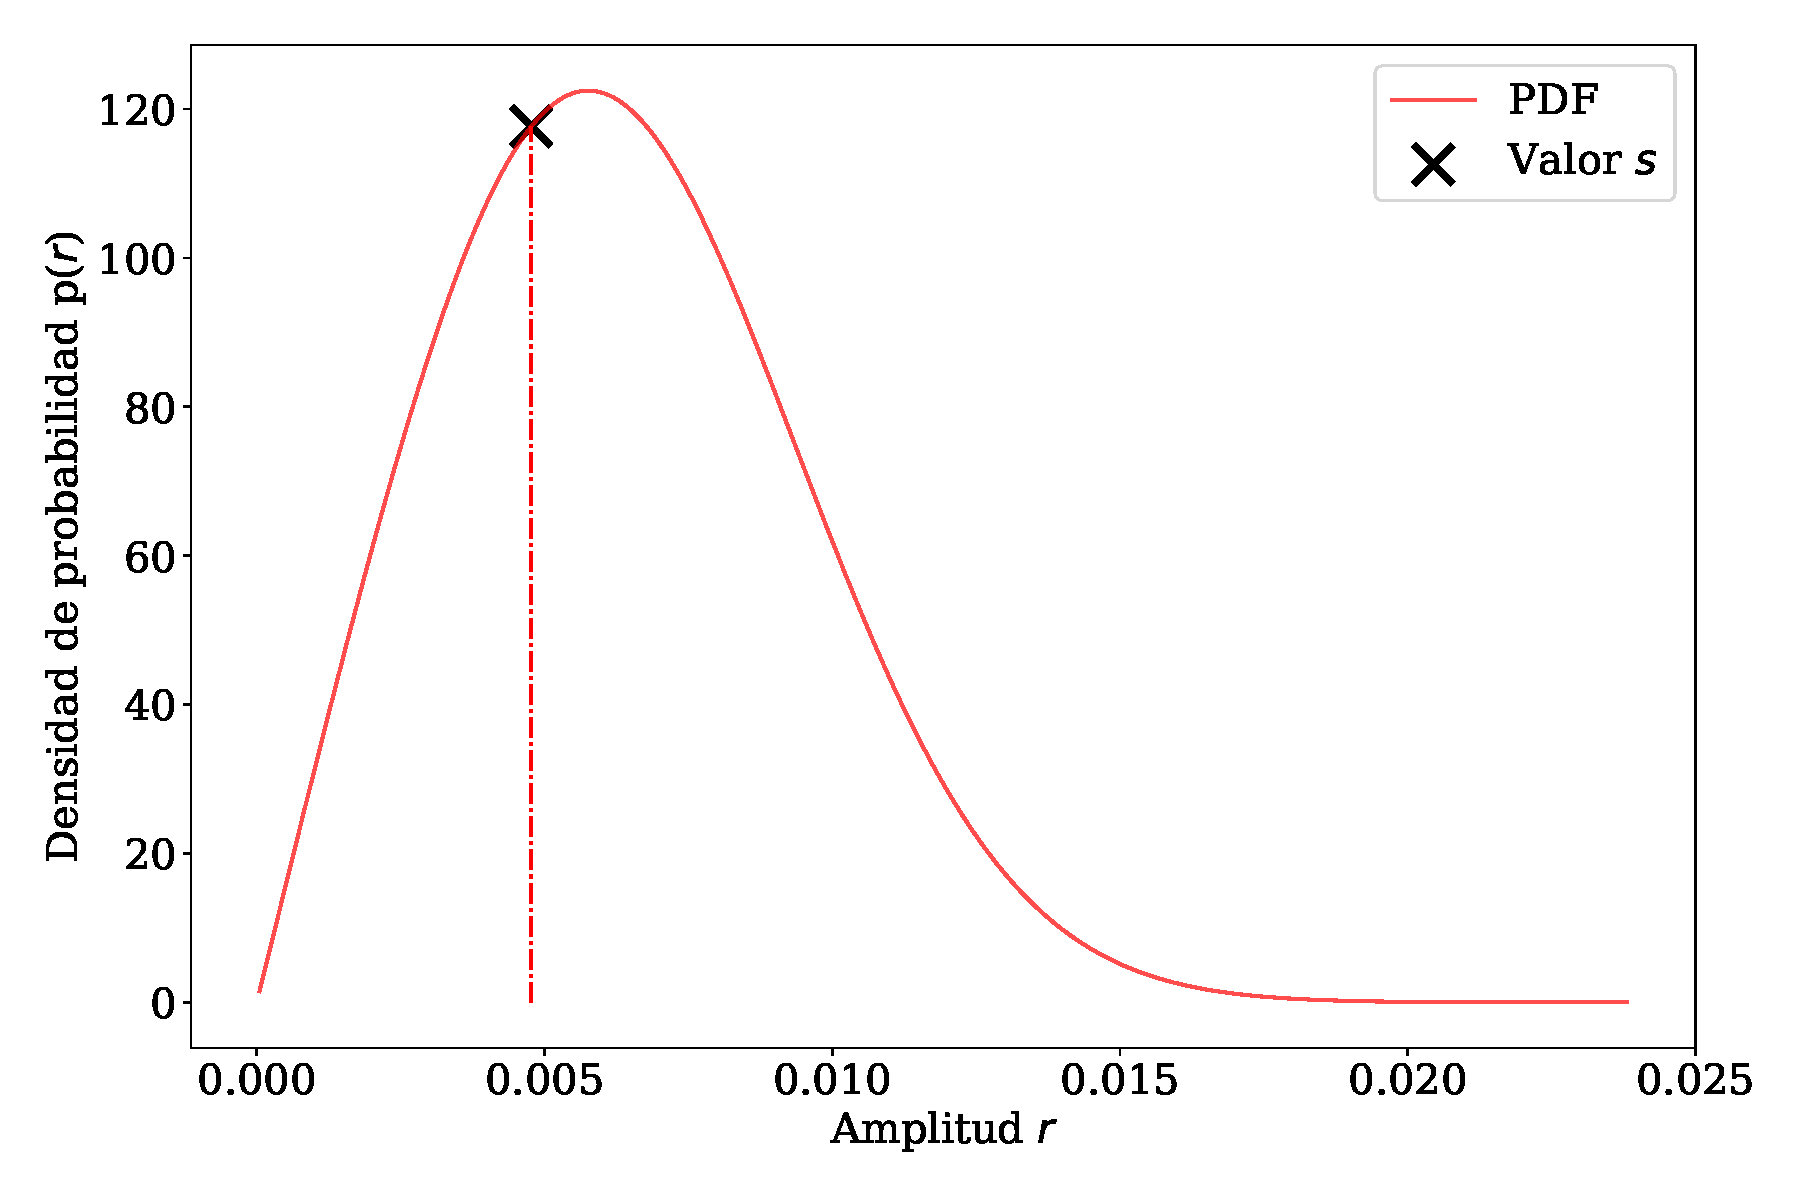
\includegraphics[width=0.75\textwidth]{bessel_prob_value_s_v2.pdf}
        \end{center}
        \caption{El gráfico de la densidad de probabilidad $p(r)$ de la amplitud $r$ para $s=0.0047$ y $\sigma=0.0038$ }
    \end{small}
\end{figure}

\subsection{Haciendo la cuenta de los márgenes de confianza de la amplitud}

Calculemos los márgenes de confianza para el ejemplo anterior de $s=0.0047$ y $\sigma=0.0038$. En este trabajo los márgenes que se obtuvieron nos dicen que el nivel de confianza en ese intervalo del $68.27\%$. Se toma este límite, dado que si $N>>1$, la distribución $p(r)$ tiende a una distribución normal y el nivel de confianza sería $1\sigma$.

Los pasos para el cálculo son los siguientes: 

\begin{enumerate}
    \item 
    Dado que la distribución tiene una función de bessel modificada de primer orden que diverge en el 0, se toma una aproximación a la función con los primeros 8 términos de la sucesión. Por lo que la función no es exacta y la norma difiere de $1$. 
    
    Para normalizar el área, se calcula la integral hasta $r_{max}=s +  10\sigma$, dado que está tan alejada del valor de amplitud obtenida, el nivel de confianza en $CL_r(0,r_{max},s)\simeq 1$, por lo que se  usa este valor para normalizar la Ec. \ref{ec:pdf} en el código.

    \item Una vez que se tiene la función normalizada, se calcula la integral de la ecuación \ref{ec:integral} $CL_r(0,s,s)$ en el intervalo  $[0,s]$ y se obtiene el valor de la función $p(s)=p_1$.

    % \item Si $CL_r(0,s,s)< 0.6827$:
    % \begin{enumerate}
        \item Teniendo en cuenta el valor inicial de $p_1$, se actualiza el valor  $p_2 \leftarrow p_1 - 0.01 p_1$ \label{itm:1}.
        \item Se calcula la integral entre los dos puntos con valores igual a $p_2$. 
        \item \label{itm:3} Si la integral es menor a $0.6827$, se repite el proceso desde el paso \ref{itm:1}. Caso contrario, si esta integral es mayor o igual a $0.6827$, se calculan los valores límites de $r$ mediante el valor $p_2$ en el paso \ref{pasofinal}. 

        La Fig.\ref{fig:itera} se muestra el área calculada en la primera iteración que se muestra verde, el valor de área obtenido no es el nivel de confianza buscada se sigue iterando hasta alcanzar el valor $p_N$, donde la integral entre esos extremos es de $0.6827$.
        \begin{figure}[H]
            \begin{small}
                \begin{center}
                    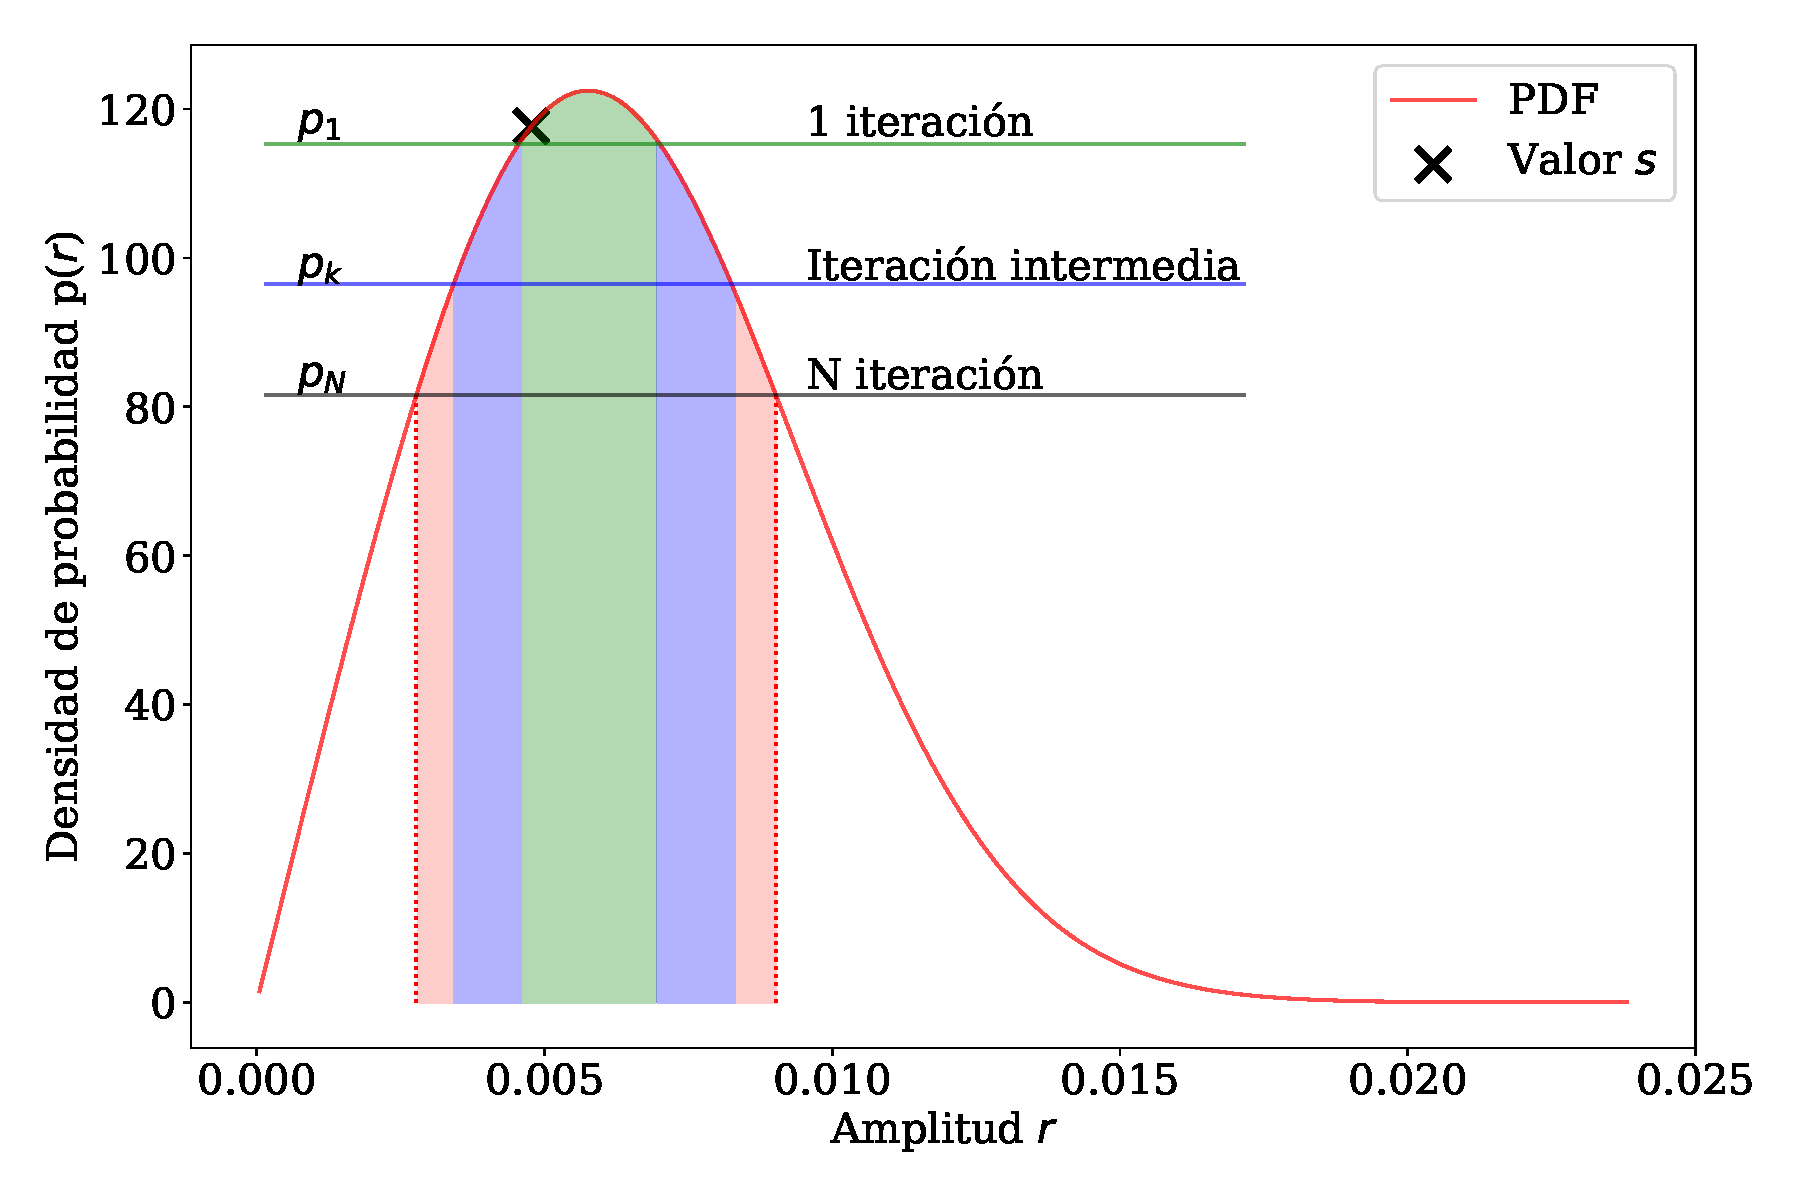
\includegraphics[width=0.75\textwidth]{bessel_prob_iterations_v2.pdf}
                \end{center}
                \caption{Iteraciones para encontrar los márgenes de confianza del $68.27\%$ de la distribución de probabilidad de la amplitud. En la N-ésima iteración se obtiene los límite de confianza buscados.}
                \label{fig:itera}
            \end{small}
            
        \end{figure}
    % \end{enumerate}
    \item Puede ocurrir que el valor de $s$ no esté entre los márgenes
     de confianza que se calcula. En este caso se toma como límite inferior $r^-$el valor $s$ y se busca el límite superior $r^+$ de tal forma que $CL(s,s+\sigma^+,s) \simeq 0.6827$.
    % \end{enumerate}
    \item \label{pasofinal} Los límites de confianza superior $r^+$  y inferior $r^-$, teniendo en cuenta el valor final $p_N$ del paso \ref{itm:3}, son tales que se cumple $p(r^+)=p(r^-)=p_N$. Finalmente los márgenes de confianza se calculan como:
    \begin{align*}
        \sigma^- = s-r^-\\
        \sigma^+ = r^+ -s
    \end{align*}
\end{enumerate}

En la Fig.\ref{margenes} se muestran los márgenes de confianza obtenidos para el ejemplo de $s=0.0047$ y $\sigma=0.0038$, el área sombreada es igual al $0.6827$
\begin{figure}[H]
    \begin{small}
        \begin{center}
            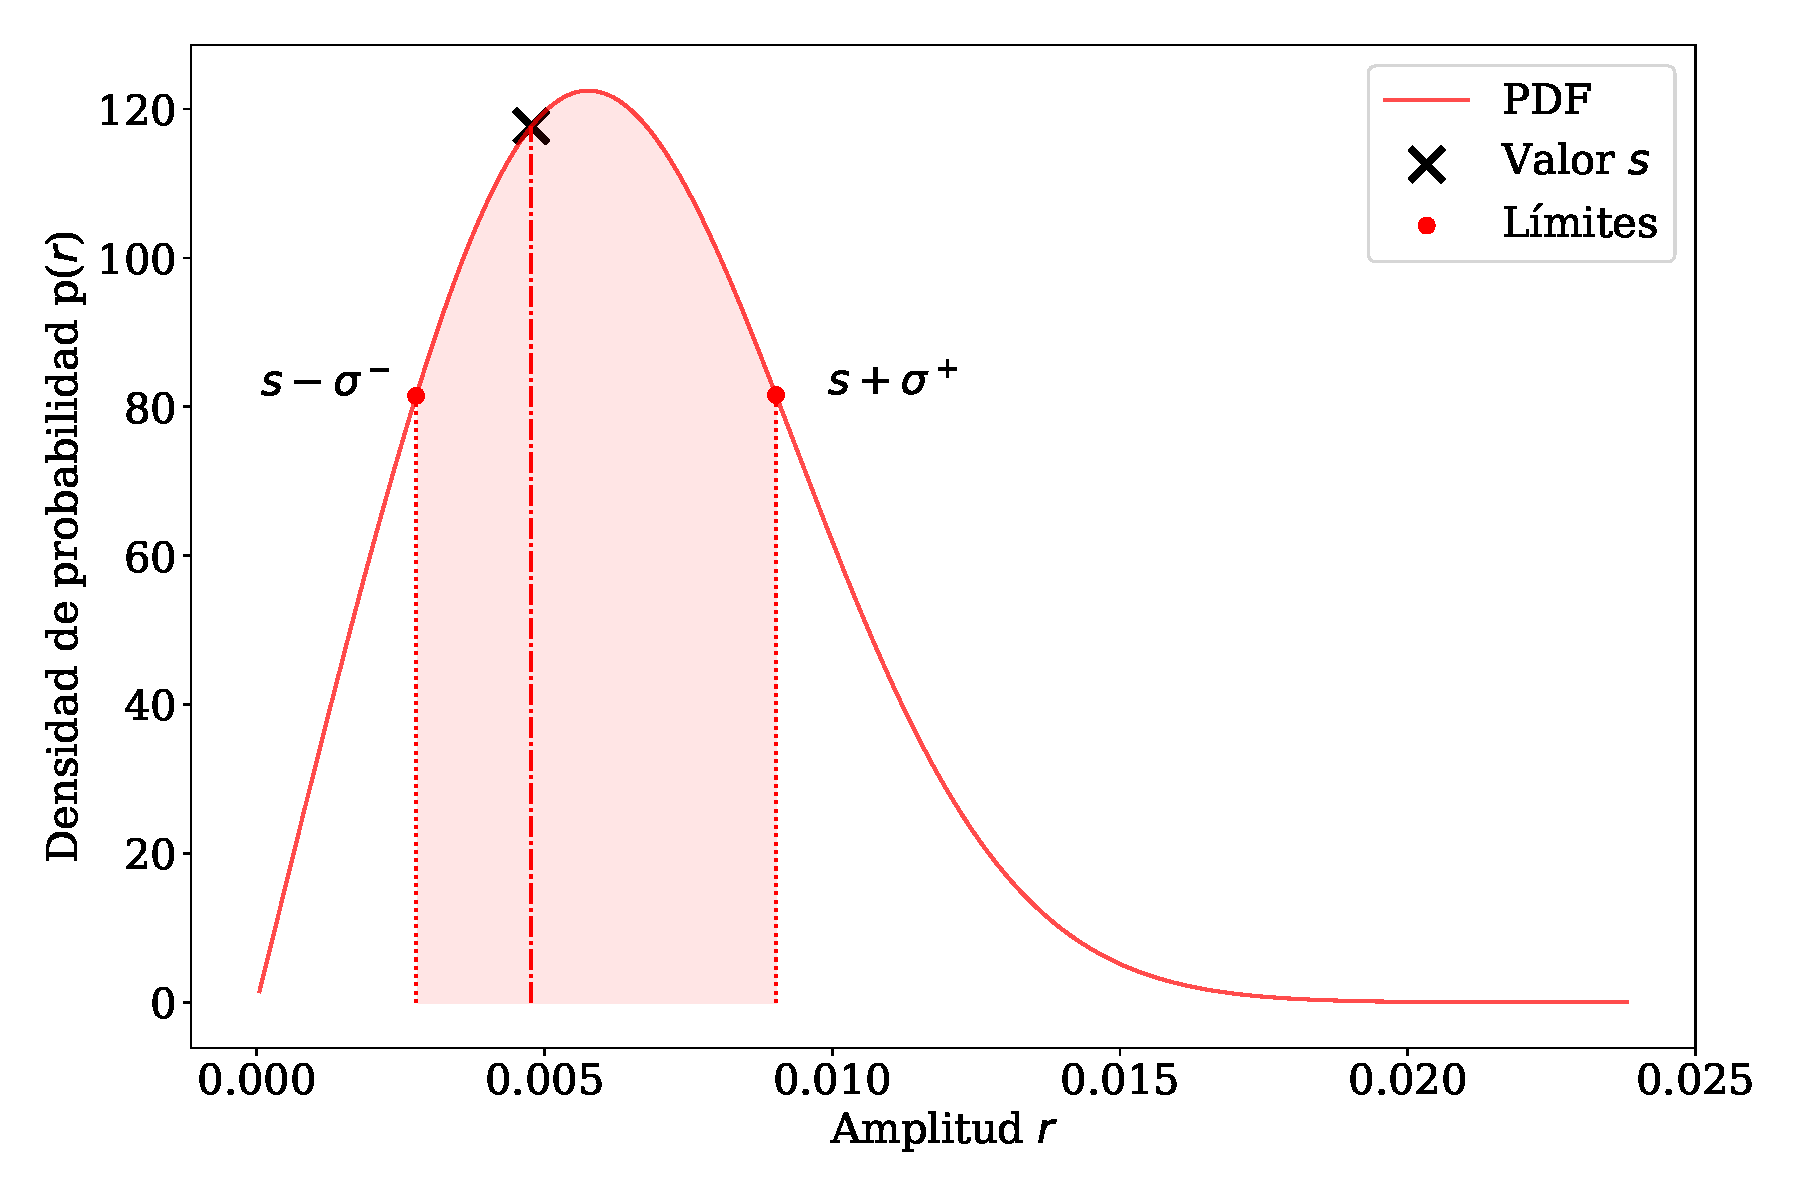
\includegraphics[width=0.75\textwidth]{bessel_prob_ej_v2.pdf}
        \end{center}
        \caption{Densidad de probabilidad de la amplitud $r$ para $s=0.0047$ y $\sigma=0.0038$. Se muestran los márgenes de confianza del $68.27\%$ }
        \label{margenes}
    \end{small}
\end{figure}

\section{Distribución de probabilidad de la fase del dipolo}

Integrando la ecuación \ref{eq:full_pdf} con respecto a $r$ en el rango $[0,\infty]$, se obtiene la distribución de probabilidad de la fase $\psi$ de la Ec.\ref{eq:phase_pdf}. Este apartado considera que las fases de la mediciones varían alrededor del cero. De esta forma, la distribución de probabilidad tiene la característica  de ser simétrica respecto a 0, por eso los límites de integración para obtener un nivel de confianza igual a 1 son $[-\pi, \pi]$.
\begin{align}
    p(\psi) &=d\psi\,\frac{1}{2\pi}e^{-k} \Bigg[ 1 + (\pi k)^{\nicefrac{1}{2}} \cos\psi e^{(k\cos^2\psi)} \Big( 1 + L \erf(L k^{\nicefrac{1}{2}} \cos\psi \Big) \Bigg ] \\ \label{eq:phase_pdf}
    CL_{\psi}(\phi_1, \phi_2, s) &= \int_{\phi_1}^{\phi_2} d\psi \, p(\psi)
\end{align}  
donde $k =\nicefrac{s^2}{2\sigma^2}$ y $\erf (x)$ es la función error, y
\begin{align*}
    L =
    \begin{cases} 
        +1 & \text{ Si } -\frac{\pi}{2} \leq x\geq \frac{\pi}{2} \\
        -1 & \text{ Caso contrario }  \\
     \end{cases}
\end{align*}

% La distribución de probabilidad tiene la característica  de ser simétrica respecto a 0, por eso los límites de integración son $[-\pi, \pi]$.

Se definió que el nivel de confianza para la fase reportada en este trabajo sea del $68.27\%$, ya que $k>>1$ la distribución de la fase se acerca a una distribución normal y este nivel de confianza es equivalente a $1\sigma_\phi$. 

Para calcular el margen de confianza $\sigma_\psi$,  dada la simetría de la función \ref{eq:phase_pdf}  con respecto al 0, se siguen los siguientes  pasos:

\begin{enumerate}
    \item Se toma un valor inicial de $\sigma_{\psi,0}=0.01$, que es equivalente a $0.57^o$.
    \item Se integra la Ec.\ref{eq:phase_pdf} en el rango $[-\sigma_{\psi,0}, \sigma_{\psi,0}]$ y se verifica si $CL_{\psi}(-\sigma_{\psi,0}, \sigma_{\psi,0},s) = 0.6827$.  Si ese es el caso, se reporta la fase como $\psi \pm \sigma_{\psi,0}$, caso contrario se vuelve al paso anterior con $\sigma_{\psi,1} \leftarrow \sigma_{\psi,0} + 0.01\sigma_{\psi,0}$. \label{paso2} y se itera hasta obtener el valor de $\sigma_{\psi,N}$ que cumpla $CL_{\psi}(-\sigma_{\psi,N}, \sigma_{\psi,N},s) = 0.6827$
\end{enumerate}

En la Fig.\ref{fig:phase_prob_ej} se muestra la distribución de probabilidad de la fase para $s=0.0047$ y $\sigma = 0.0038$, también se incluye los límites de confianza obtenidos.

\begin{figure}[H]
    \begin{small}
        \begin{center}
            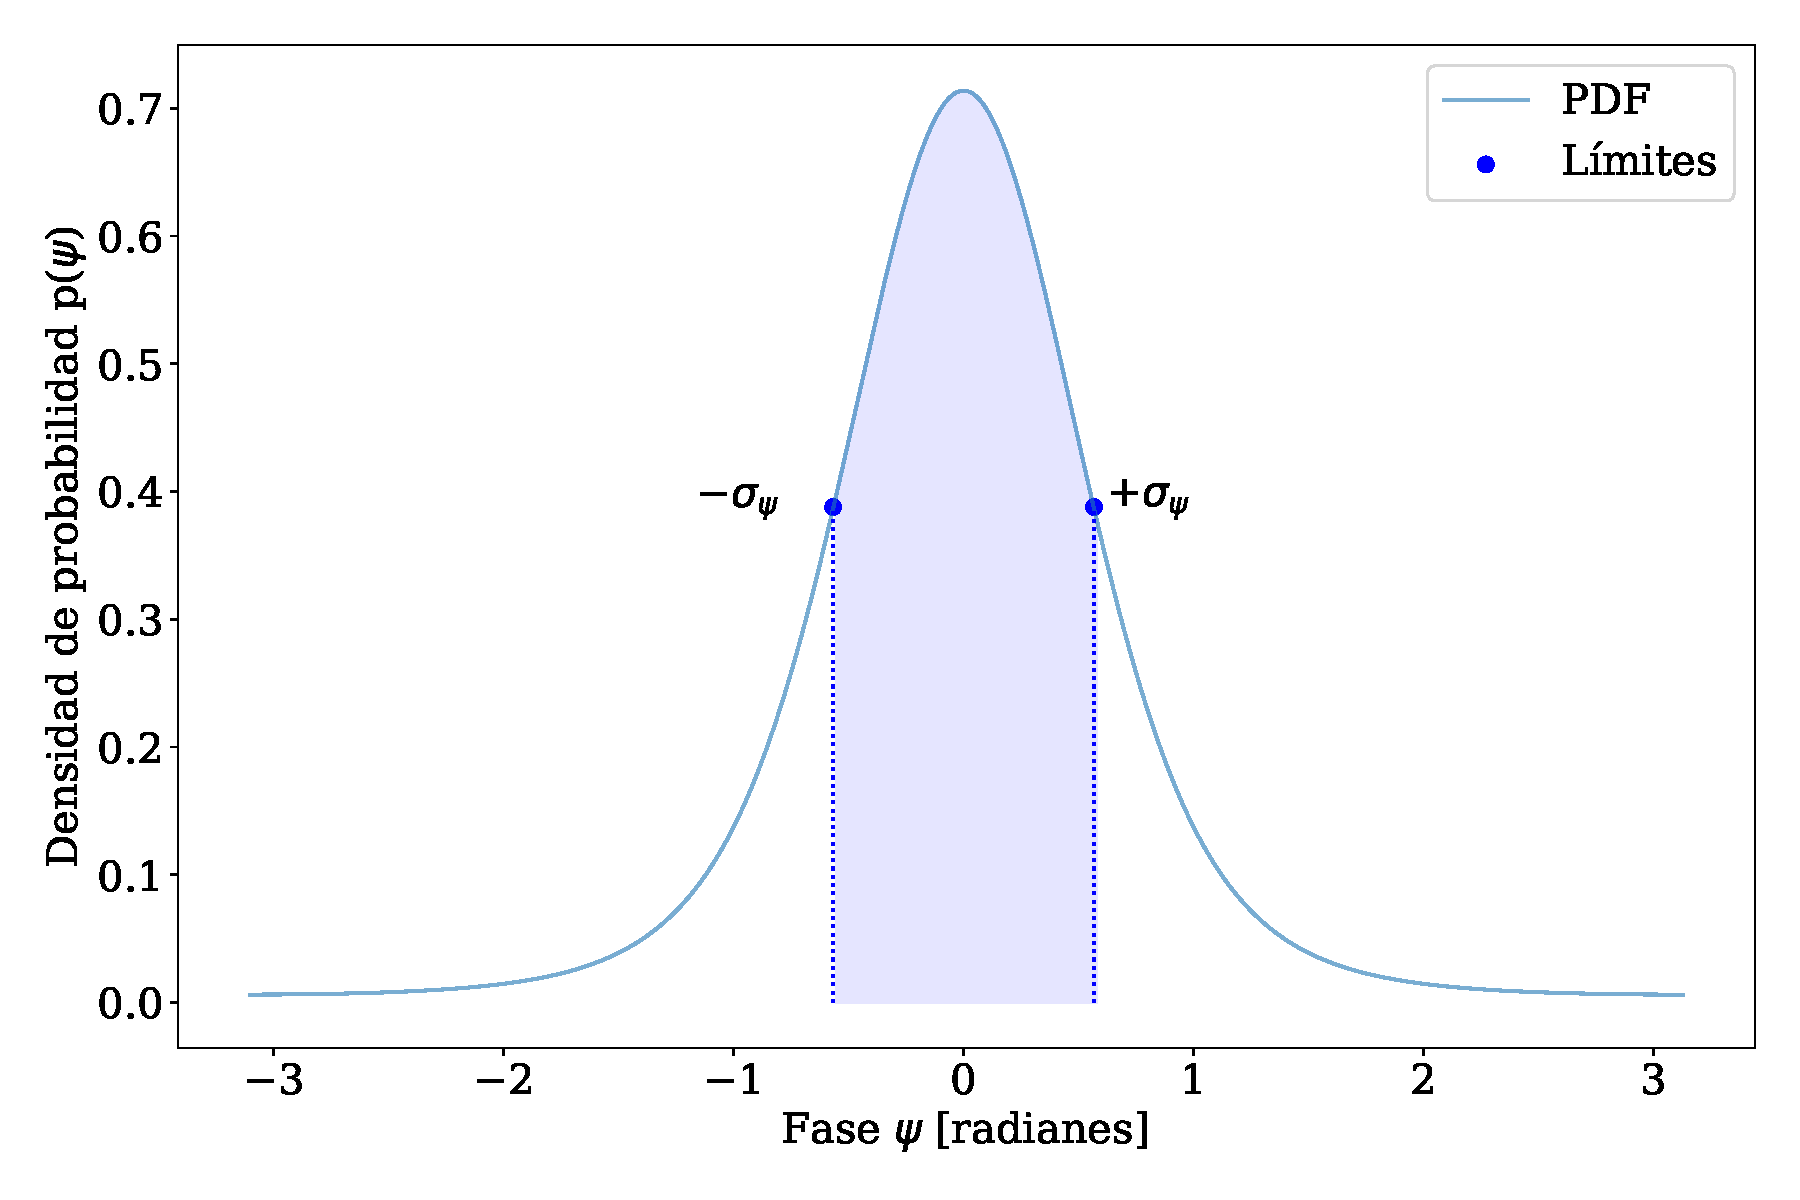
\includegraphics[width=0.75\textwidth]{phase_prob_ej_v2.pdf}
        \end{center}
        \caption{La distribución de probabilidad de la fase $\psi$ para $s=0.0047$ y $\sigma = 0.0038$ con los márgenes de confianza del $68.27\%$.}
        \label{fig:phase_prob_ej}
    \end{small}
\end{figure}


\chapter{Resultados del método East - West}

En este capítulo se presentan los resultados obtenidos mediante el método East-West con los eventos de Todos los Disparos en distintos rangos de energía. Estos resultados se comparan con los valores obtenidos en \cite{Aab_2020} sobre los eventos  del Disparo Estándar. 
% \section{Tabla cantidad de eventos para distintos rangos de energía}

Los eventos son clasificados en los distintos rangos con la energía reportada el conjunto de eventos registrados mediante de todos los disparos  entre el 2014 y 2019 y para el disparo estándar entre el 2004 y 2018.

\begin{table}[H]
    \begin{small}
        \begin{center}
            \begin{tabular}{lc|l|l|l|}
\hline
\multicolumn{1}{|l|}{\multirow{4}{*}{\begin{tabular}[c]{@{}c@{}}Rango \\ Tiempo\end{tabular}}}    & Todos       & Inicio &\multicolumn{2}{l|}{1 de Enero, 2014 } \\ \cline{3-5} 
\multicolumn{1}{|l|}{}                                                                            & 6 años      & Fin    &\multicolumn{2}{l|}{1 de Enero, 2020} \\ \cline{2-5} 
\multicolumn{1}{|l|}{}                                                                            & Estándar    & Inicio &\multicolumn{2}{l|}{1 de Enero, 2004} \\ \cline{3-5}
\multicolumn{1}{|l|}{}                                                                            & 14.8 años   & Fin    &\multicolumn{2}{l|}{1 de Octubre, 2018} \\ \hline  \\

\hline                                                                          \multicolumn{2}{|c|}{Rango [EeV]}                                                    & \multicolumn{1}{c|}{0.25 - 0.5}  & \multicolumn{1}{c|}{ 0.5  - 1 } &\multicolumn{1}{c|}{ 1 - 2 } \\ \hline
\multicolumn{1}{|l|}{\multirow{2}{*}{Eventos}}                            & Todos    & $3\,967\,368$     & $3\,638\,226$   & $1\,081\,846$ \\ \cline{2-5} 
\multicolumn{1}{|l|}{}                                                    & Estándar & $770\,323$        & $2\,388\,468$   & $1\,243\,098$ \\ \hline
\multicolumn{1}{|l|}{\multirow{2}{*}{\begin{tabular}[c]{@{}c@{}}Energía \\ Media\end{tabular}}} & Todos    & $0.38$           & $0.69$         & $1.32$       \\ \cline{2-5} 
\multicolumn{1}{|l|}{}                                                                             & Estándar & $0.42$            & $0.71$          & $1.34$       \\ \hline
\end{tabular}
            \caption{Tabla de eventos por rango de energía }
            \label{tab:}
        \end{center}
    \end{small}
\end{table}



\section{Resultados en distintos rangos de energía}
\subsection{Resultados en el rango 0.25 EeV - 0.5 EeV}

En la Fig. \ref{fig:primer} se comparan las direcciones en las que apuntan la fase en frecuencia sidérea obtenida en este trabajo con la obtenida en \cite{Aab_2020}. 
Las fases tiene un margen donde se solapan en la incertidumbre pero no son comparables, la línea punteada marca la dirección del centro galáctico.
\begin{table}[H]
    \begin{small}
        \begin{center}
            \begin{tabular}[c]{l|c|c||c|}
\cline{2-4}                                       & \multicolumn{2}{c||}{Todos los disparos}    & \multicolumn{1}{c|}{Disparo Estándar}   \\ \hline
\multicolumn{1}{|l|}{Frecuencia:                } & Solar	                & Sidérea	                & Sidérea \cite{Aab_2020}   \\ \hline
\multicolumn{1}{|l|}{Amplitud r [\%]:           } & $0.17^{+0.22}_{-0.07}$	& $0.12^{+0.24}_{-0.03}$ 	& $0.5^{+0.4}_{-0.2}$ \cite{codigo}      \\
\multicolumn{1}{|l|}{$r_{99}$ [\%]:             } & \multicolumn{2}{c||}{0.58}                          & 1.1\cite{codigo}                 \\
\multicolumn{1}{|l|}{$r^{UL}$ [\%]:             } & 0.67 	                & 0.64                      & 1.4\cite{codigo}                 \\ 
\multicolumn{1}{|l|}{$\sigma$[\%]:              } & \multicolumn{2}{c||}{0.19}                          & 0.38\cite{codigo}       \\\hline
\multicolumn{1}{|l|}{Amplitud $d_\perp$[\%]:    } & -	                    & $0.16^{+0.31}_{-0.04}$ 	& $0.6^{+0.5}_{-0.3}$       \\
\multicolumn{1}{|l|}{$d_{99}$ [\%]:             } & - 	                    & 0.73                      & 1.5  \cite{codigo}                \\
\multicolumn{1}{|l|}{$d_{\perp}^{UL}[\%]$       } & -                       & 0.80                      & 1.8                         \\
\multicolumn{1}{|l|}{$\sigma_{x,y}$[\%]:        } & -	                    & 0.24	                    & 0.48       \\\hline
\multicolumn{1}{|l|}{Probabilidad      :        } & 0.66                    & 0.81	                    & 0.45       \\
\multicolumn{1}{|l|}{Fase[$^o$]:                } & 221$\pm$93              & 280$\pm$124                & 225$\pm$64\\ \hline
\multicolumn{1}{|l|}{$\langle\cos\delta \rangle$} & \multicolumn{2}{c||}{0.79}        	                & 0.79 \cite{codigo}        \\        
\multicolumn{1}{|l|}{$\langle\sin\theta \rangle$} & \multicolumn{2}{c||}{0.46}        	                & 0.52 \cite{codigo}        \\ \hline       
            \end{tabular}
        \end{center}
    \end{small}
    \caption{Características para las frecuencias solar y sidérea con el método East-West en el primer armónico en rango de energía 0.25 EeV - 0.5 EeV.}
    \label{tab:solar}
\end{table}


Realizando el barrido de frecuencias con la variable de la Ec.\ref{ra_arb}, se obtiene que en este rango de energía las amplitudes se  distribuyen en frecuencia como se muestra en la Fig.\ref{fig:primer_barrido}. La línea horizontal indica el valor de $r_{99}$ para cada frecuencia, además se observa que ninguna frecuencia supera dicho umbral.

\begin{figure}[H]
    \begin{small}
        \begin{center}
            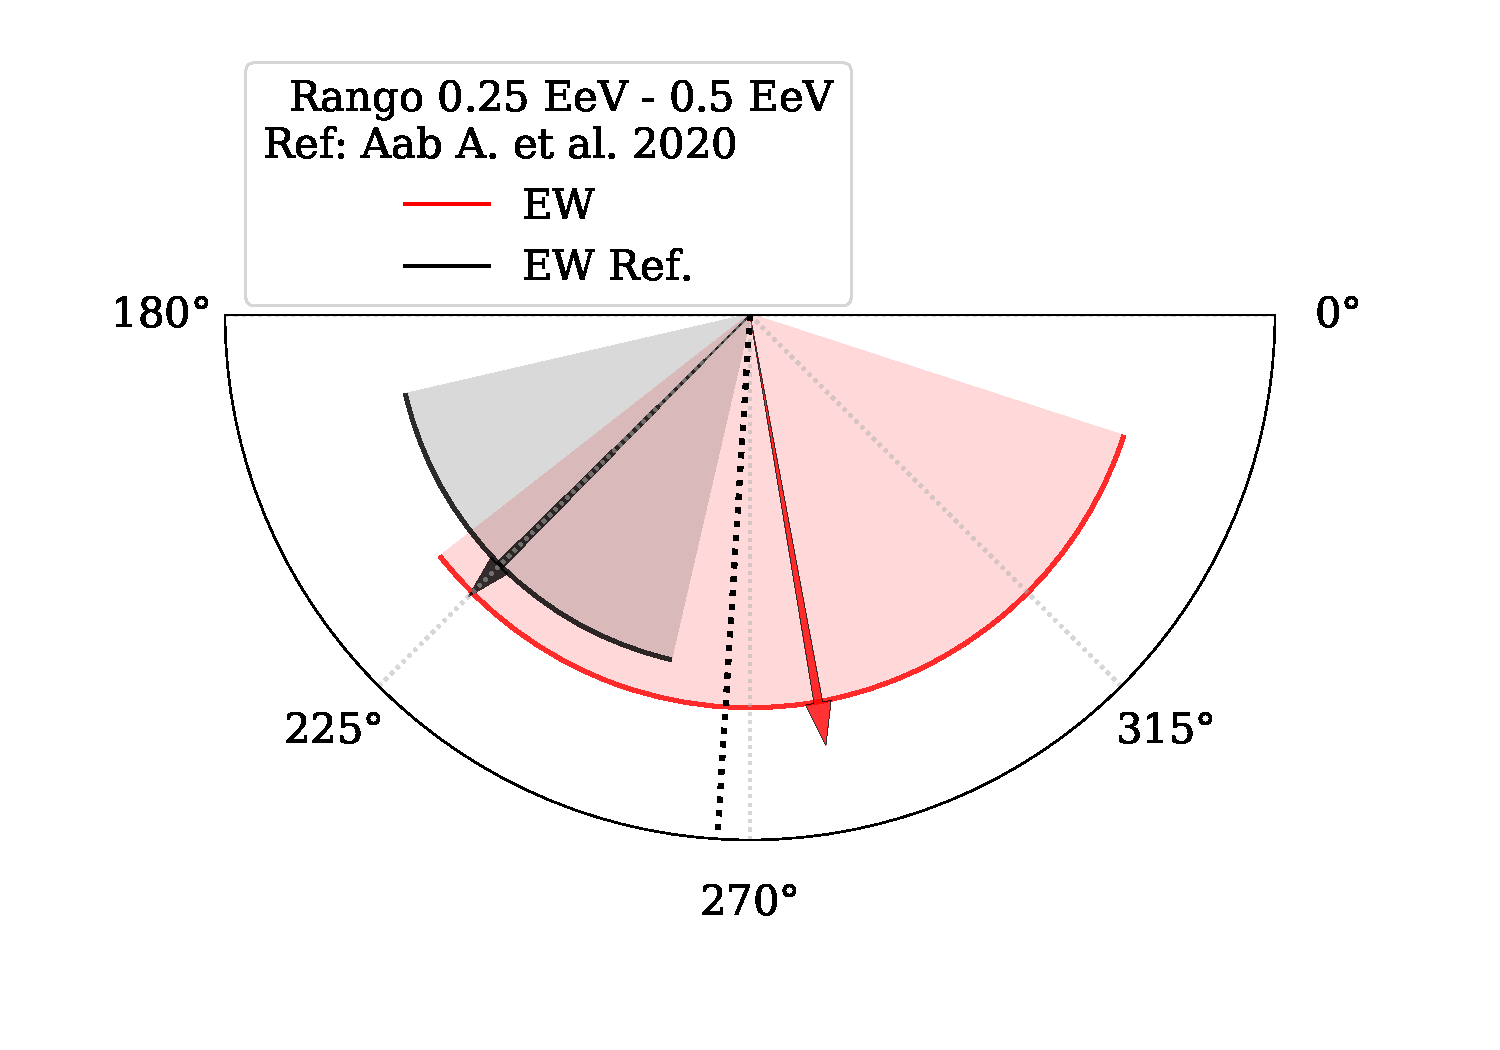
\includegraphics[width=0.75\textwidth]{phase_primer_bin_v2.pdf}
        \end{center}
        \caption{Valores de las fases obtenidos en este trabajo y en la referencia con sus respectivas incertidumbres para la frecuencia sidérea en el  rango 0.25 EeV - 0.5 EeV .}
        \label{fig:primer}
    \end{small}
\end{figure}

\begin{figure}[H]
    \begin{small}
        \begin{center}
            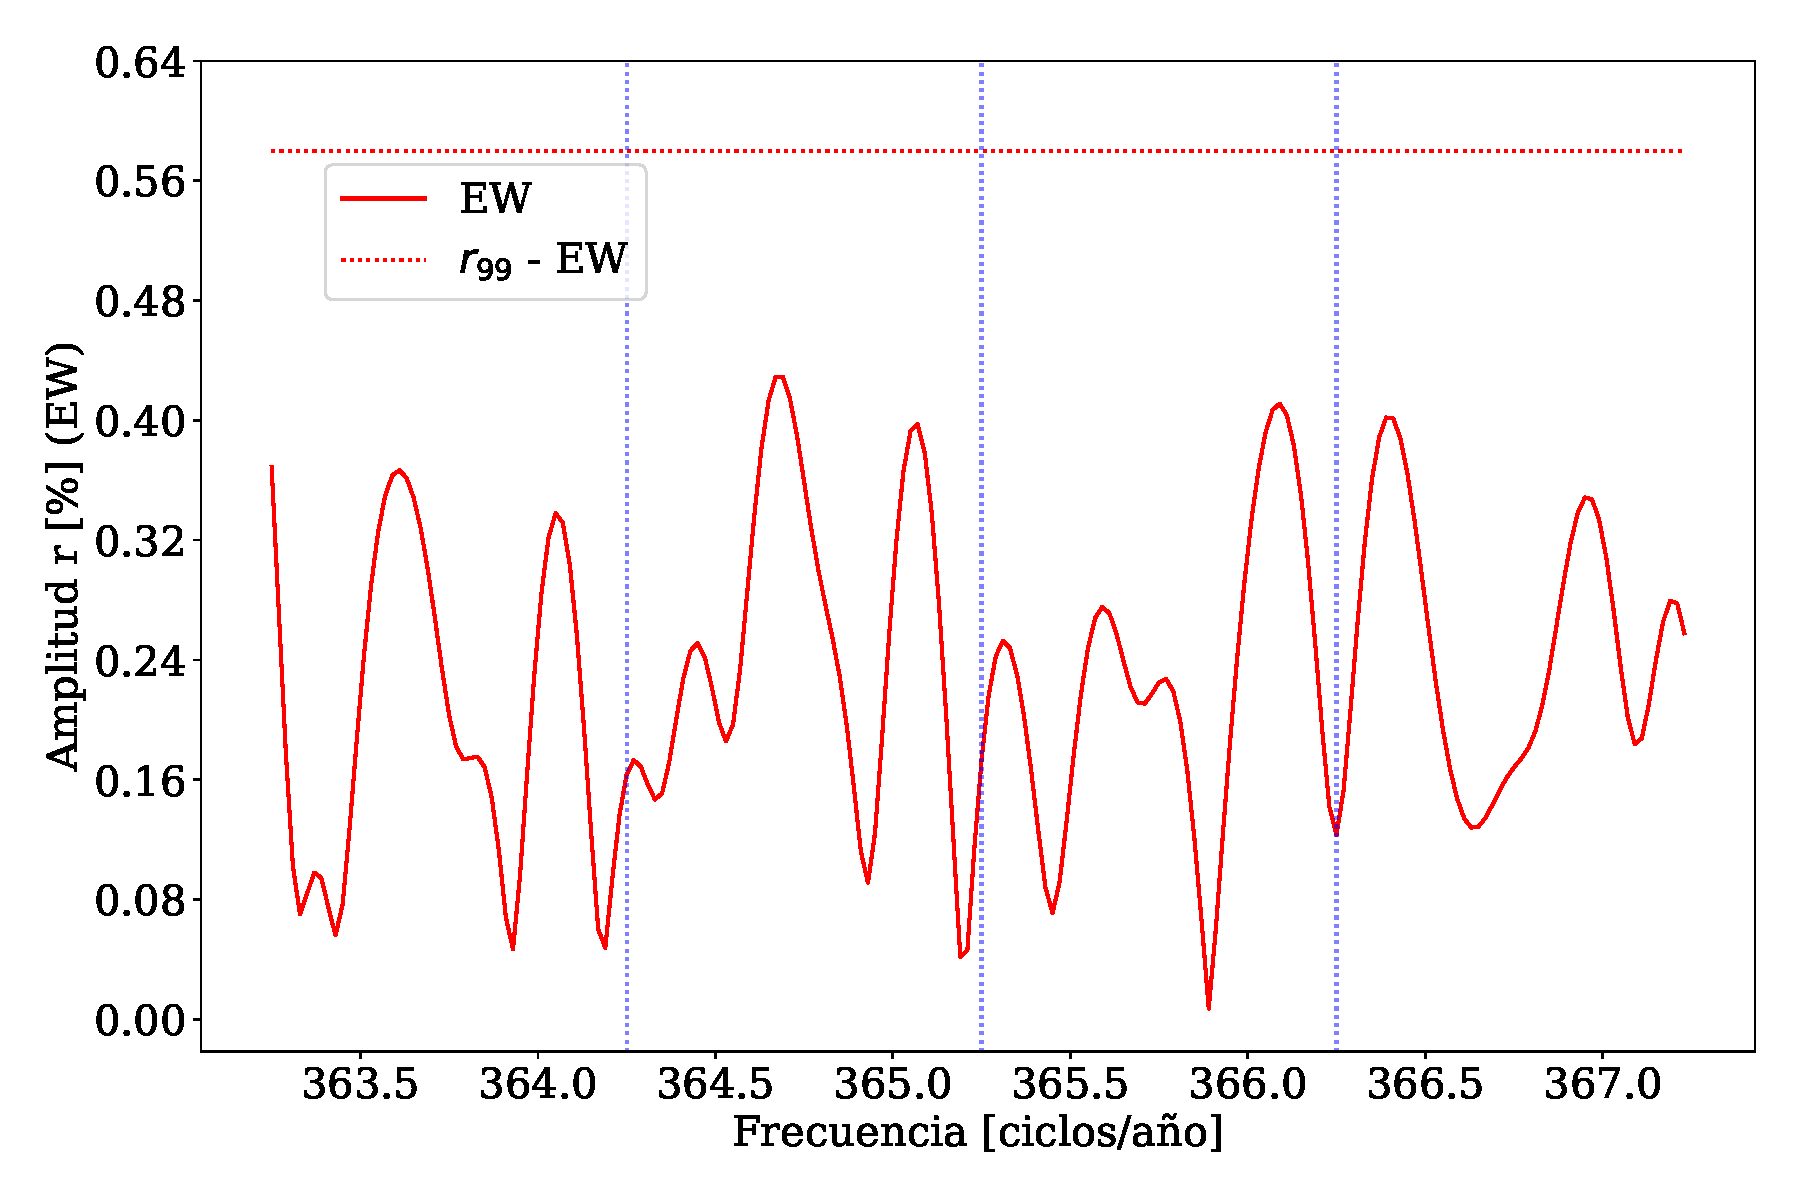
\includegraphics[width=0.75\textwidth]{plot_bin_1_barrido_v3_EW.pdf}
        \end{center}
        \caption{Barrido de frecuencias en el  rango 0.25 EeV - 0.50 EeV .}
        \label{fig:primer_barrido}
    \end{small}
\end{figure}

\subsection{Resultados en el rango 0.5 EeV - 1 EeV}
En este rango de energía se observa una diferencia entre las probabilidades de este trabajo y \cite{Aab_2020}  ne la frecuencia sidérea. Este valor dice cuando probable es que las amplitudes sean debido al ruido. Este trabajo obtiene que la amplitud en sidérea es significativa por un  $6\%$.  

En la Fig. \ref{fig:segundo} se comparan las direcciones en las que apuntan la fase en frecuencia sidérea obtenida en este trabajo con la obtenida en \cite{Aab_2020}. En esta figura se observa que las fases son comparables entre sí y apuntan a una dirección cercana al centro galáctico (línea punteada).

El barrido de frecuencias con la variable de la Ec.\ref{ra_arb} para este rango de energía se observa en la Fig.\ref{fig:segundo_barrido}. La línea horizontal indica el valor de $r_{99}$ para cada frecuencia, además se observa que ninguna frecuencia supera dicho umbral. Otro aspecto es que la zona de la frecuencia anti-sidérea no tiene picos pronunciados, como en la frecuencia solar o sidérea.

\begin{figure}[H]
    \begin{small}
        \begin{center}
            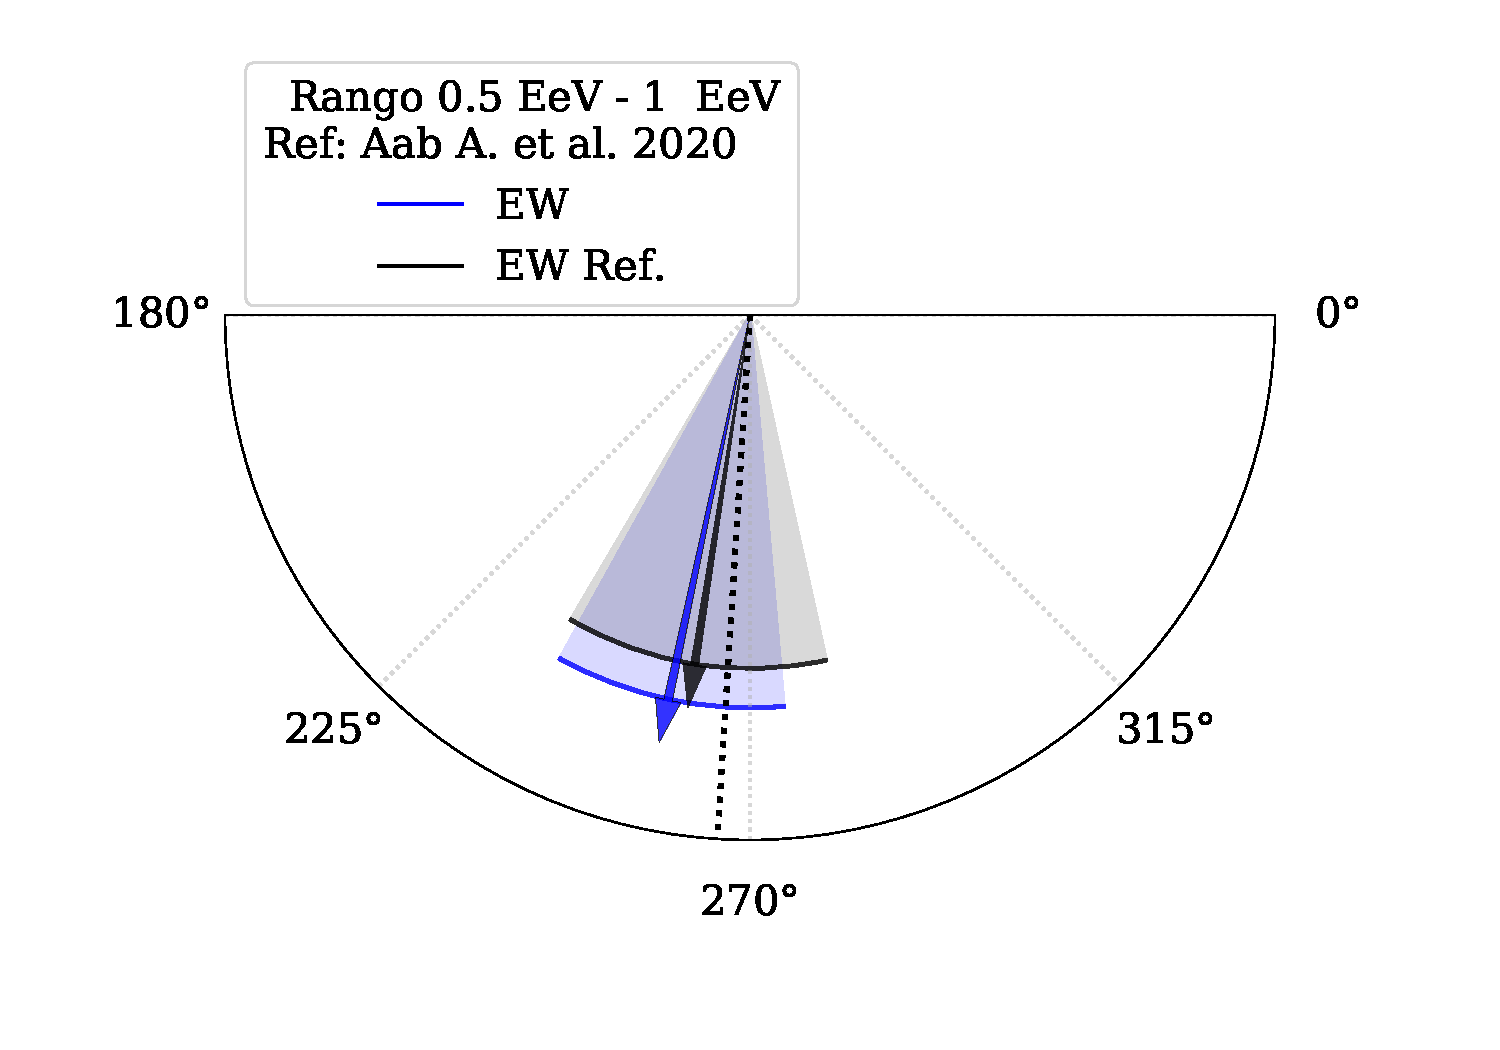
\includegraphics[width=0.75\textwidth]{phase_segundo_bin_v2.pdf}
        \end{center}
        \caption{Valores de las fases obtenidos en este trabajo y en la referencia con sus respectivas incertidumbres para la frecuencia sidérea en el  rango 0.5 EeV - 1.0 EeV .}
        \label{fig:segundo}
    \end{small}
\end{figure}

\begin{table}[H]
        \begin{small}
            \begin{center}
                \begin{tabular}[c]{l|c|c||c|}
\cline{2-4}                                       & \multicolumn{2}{c||}{Todos los disparos}    & \multicolumn{1}{c|}{Disparo Estándar}   \\ \hline
\multicolumn{1}{|l|}{Frecuencia:                } & Solar	                & Sidérea	                & Sidérea \cite{Aab_2020}   \\ \hline
\multicolumn{1}{|l|}{Amplitud r [\%]:           } & $0.43^{+0.21}_{-0.14}$	& $0.44^{+0.21}_{-0.14}$ 	& $0.38^{+0.20}_{-0.14}$ \cite{codigo}      \\
\multicolumn{1}{|l|}{$r_{99}$ [\%]:             } & \multicolumn{2}{c||}{0.56}                         & 0.64\cite{codigo}                 \\
\multicolumn{1}{|l|}{$r^{UL}$ [\%]:             } & 0.89 	                & 0.90                      & 0.90 \cite{codigo}                 \\ 
\multicolumn{1}{|l|}{$\sigma$[\%]:              } & \multicolumn{2}{c||}{0.18}                         & 0.21 \cite{codigo}      \\\hline
\multicolumn{1}{|l|}{Amplitud $d_\perp$[\%]:    } & -	                    & $0.56^{+0.27}_{-0.18}$ 	& $0.5^{+0.3}_{-0.2}$       \\
\multicolumn{1}{|l|}{$d_{99}$ [\%]:             } & - 	                    & 0.71                      & 0.8   \cite{codigo}                \\
\multicolumn{1}{|l|}{$d_{\perp}^{UL}[\%]$       } & -                       & 1.1                       & 1.1                         \\
\multicolumn{1}{|l|}{$\sigma_{x,y}$[\%]:        } & -	                    & 0.23	                    & 0.21       \\\hline
\multicolumn{1}{|l|}{Probabilidad      :        } & 0.065                   & 0.055	                    & 0.20       \\
\multicolumn{1}{|l|}{Fase[$^o$]:                } & 205$\pm$35              & 258$\pm$34                & 261$\pm$43\\ \hline
\multicolumn{1}{|l|}{$\langle\cos\delta \rangle$} & \multicolumn{2}{c||}{0.79}        	                & 0.79 \cite{codigo}        \\        
\multicolumn{1}{|l|}{$\langle\sin\theta \rangle$} & \multicolumn{2}{c||}{0.50}        	                & 0.54\cite{codigo}        \\ \hline       
                \end{tabular}
            \end{center}
        \end{small}
        \caption{Características para las frecuencias solar y sidérea con el método East-West en el primer armónico en rango de energía 0.5 EeV - 1 EeV}
        \label{tab:solar}
    \end{table}


    \begin{figure}[H]
        \begin{small}
            \begin{center}
                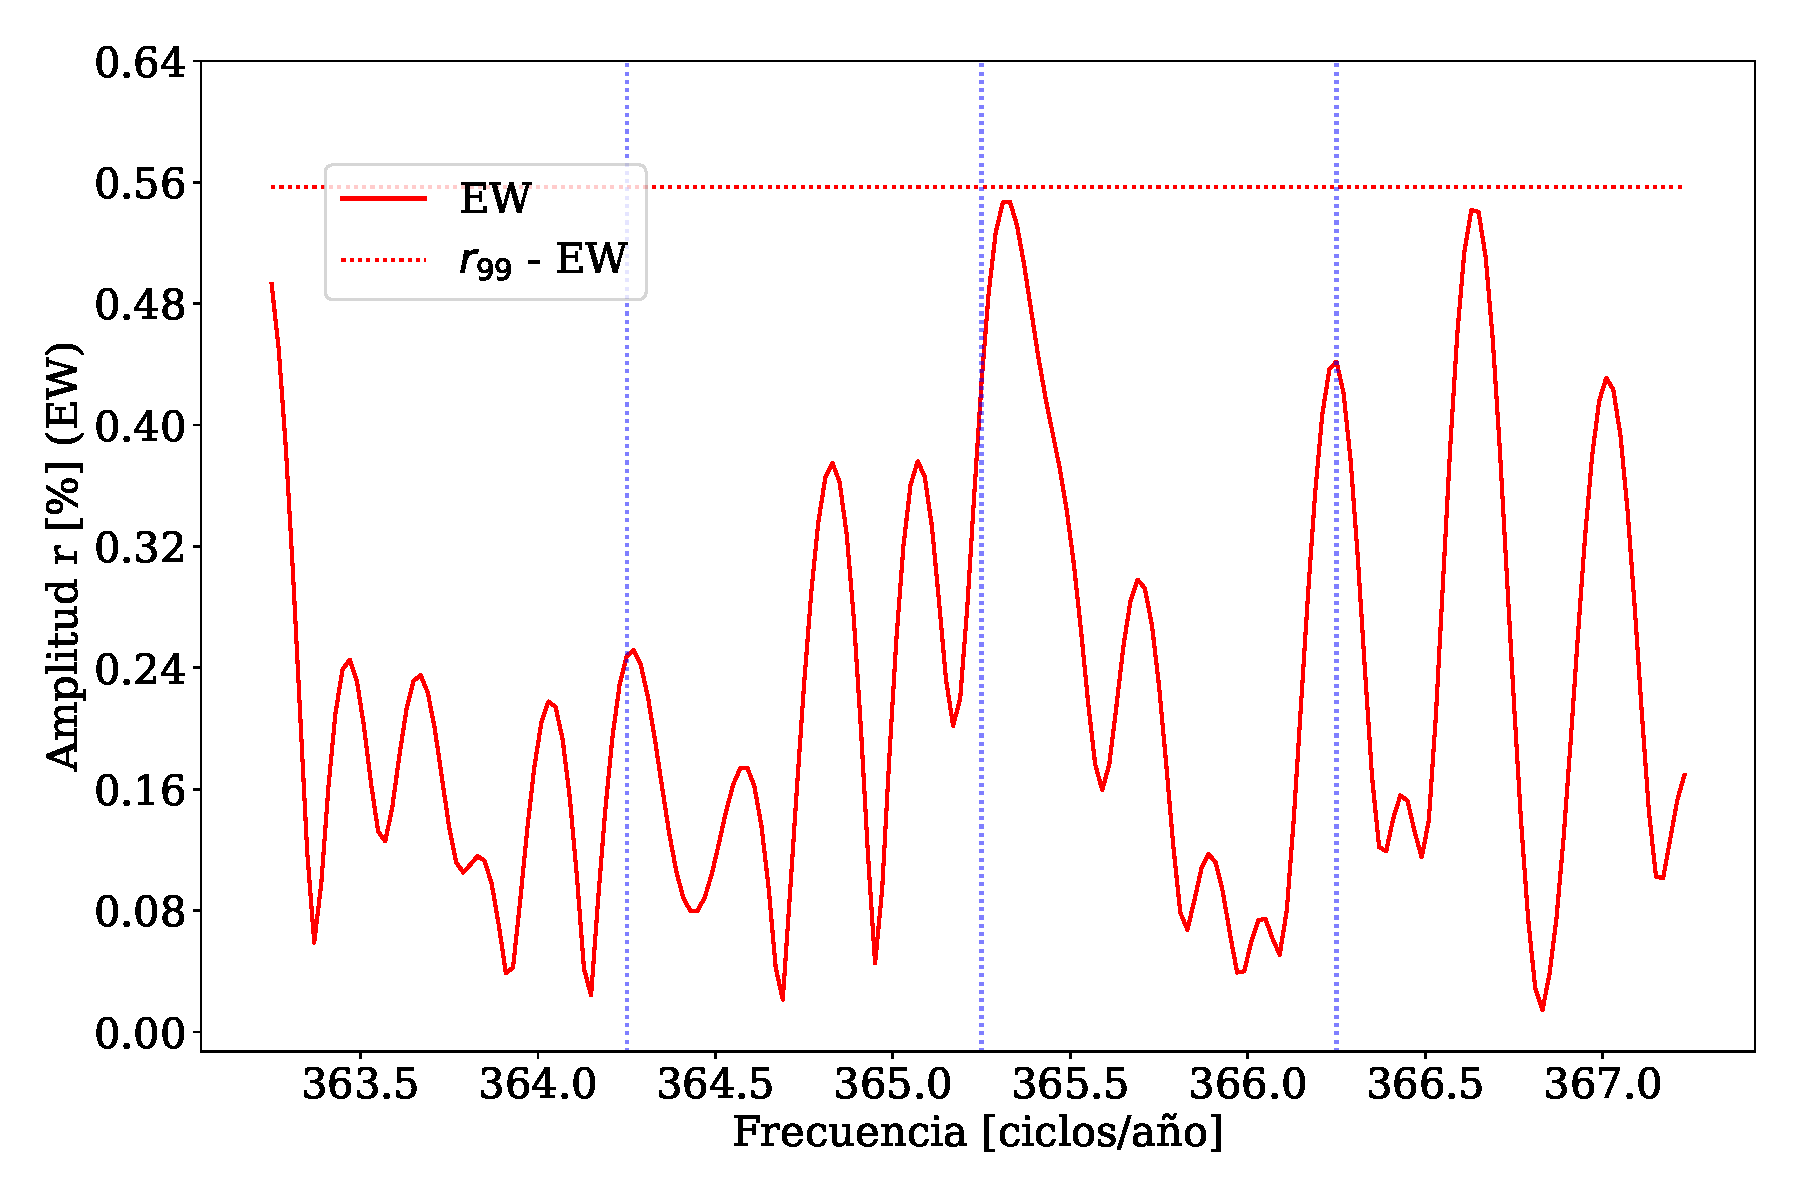
\includegraphics[width=0.75\textwidth]{plot_bin_2_barrido_v3_EW.pdf}
            \end{center}
            \caption{Barrido de frecuencias en el  rango 0.5 EeV - 1.0 EeV .}
            \label{fig:segundo_barrido}
        \end{small}
    \end{figure}    


\subsection{Resultados en el rango 1 EeV - 2 EeV}

 
En las Tablas \ref{tab:solar_3} y \ref{tab:siderea_3} se comparan los resultados de este trabajo y los obtenidos en \cite{Aab_2020} para la frecuencia solar y sidérea respectivamente. En el Fig.\ref{fig:tercer} se observan en un gráfico polar las fases de la referencia y este trabajo para la frecuencia sidérea. Los resultados son comparables entre sí.
    
    \begin{table}[H]
        \begin{small}
            \begin{center}
                \begin{tabular}[c]{l|c|c|}
                    \cline{2-3}         & \multicolumn{2}{c|}{Todos los disparos} \\ \cline{2-3}
                                        & Rayleigh                      & East - West            \\\hline
\multicolumn{1}{|l|}{Frecuencia:}             &\multicolumn{2}{c|}{Solar}        \\
\multicolumn{1}{|l|}{Amplitud $r$[\%]:} & $0.24^{+0.16}_{-0.09}$        & $0.28^{+0.35}_{-0.11}$ \\
\multicolumn{1}{|l|}{$r_{99}$ [\%]:   } & 0.41                          & 0.91       \\
\multicolumn{1}{|l|}{$r_{UL}$ [\%]:   } & 0.58                          & 1.1       \\
\multicolumn{1}{|l|}{$\sigma$:        } & 0.14                          & 0.30          \\\hline
\multicolumn{1}{|l|}{Probabilidad:    } & 0.22                          & 0.65          \\
\multicolumn{1}{|l|}{Fase:            } & 260$\pm$48                    & 279$\pm$90    \\\hline
                \end{tabular}
            \end{center}
        \end{small}
        \caption{Características para la frecuencia solar con los métodos de Rayleigh  e East-West en el primer armónico.}
        \label{tab:solar_3}
    \end{table}

    \begin{table}[H]
        \begin{small}
            \begin{center}
                \begin{tabular}[c]{l|c|c||c|}
                    \cline{2-4}               &  \multicolumn{2}{c||}{Todos los Disparos}                  & Disparo Estándar      \\
                    \cline{2-4}               & Rayleigh                      & East - West                 & East - West\cite{Aab_2020}      \\\hline
\multicolumn{1}{|l|}{Frecuencia:             }& \multicolumn{2}{c||}{Sidérea}                               & Sidérea        \\ \hline
\multicolumn{1}{|l|}{Amplitud $r$ [\%]:      }& $0.32^{+0.16}_{-0.10}$ 	      & $0.5^{+0.3}_{-0.2}$         & $0.14^{+0.37}_{-0.02}$\cite{codigo}       \\
\multicolumn{1}{|l|}{$r_{99}$[\%]:           }& 0.41	                      & 0.91                        & 0.84\cite{codigo}        \\
\multicolumn{1}{|l|}{$r^{UL}[\%]$      }      & 0.66                          & 1.3                         & 0.89 \cite{codigo}        \\
\multicolumn{1}{|l|}{$\sigma$[\%]:     }      & 0.14                          & 0.30	                    & 0.28 \cite{codigo}          \\ \hline
\multicolumn{1}{|l|}{Amplitud $d_\perp$ [\%]:}& $0.41^{+0.20}_{-0.13}$        & $0.6^{+0.4}_{-0.3}$         & $0.18^{+0.47}_{-0.02}$       \\ 
\multicolumn{1}{|l|}{$d_{99}$[\%]:           }& 0.53	                      & 1.1                         & 1.1\cite{codigo}        \\
\multicolumn{1}{|l|}{$d_{\perp}^{UL}[\%]$    }& 0.84                          & 1.6                         & 1.1        \\
\multicolumn{1}{|l|}{$\sigma_{x,y}$[\%]:     }& 0.17                          & 0.38	                    & 0.35          \\ \hline
\multicolumn{1}{|l|}{Probabilidad:           }& 0.063	                      & 0.26                        & 0.87          \\
\multicolumn{1}{|l|}{Fase[$^o$]:             }& 357$\pm$35                    & 320$\pm$50                 & 291$\pm$100      \\\hline
\multicolumn{1}{|l|}{$\langle\cos\delta\rangle$} & \multicolumn{2}{c||}{0.78}                              & 0.78       \\        
\multicolumn{1}{|l|}{$\langle\sin\theta\rangle$} & \multicolumn{2}{c||}{0.55}                              & 0.57       \\ \hline       
\end{tabular}
            \end{center}
        \end{small}
        \caption{Características para la frecuencia sidérea con los métodos de Rayleigh  e East-West en el primer armónico.}
        \label{tab:siderea_3}
    \end{table}
   
    \begin{figure}[H]
        \begin{small}
            \begin{center}
                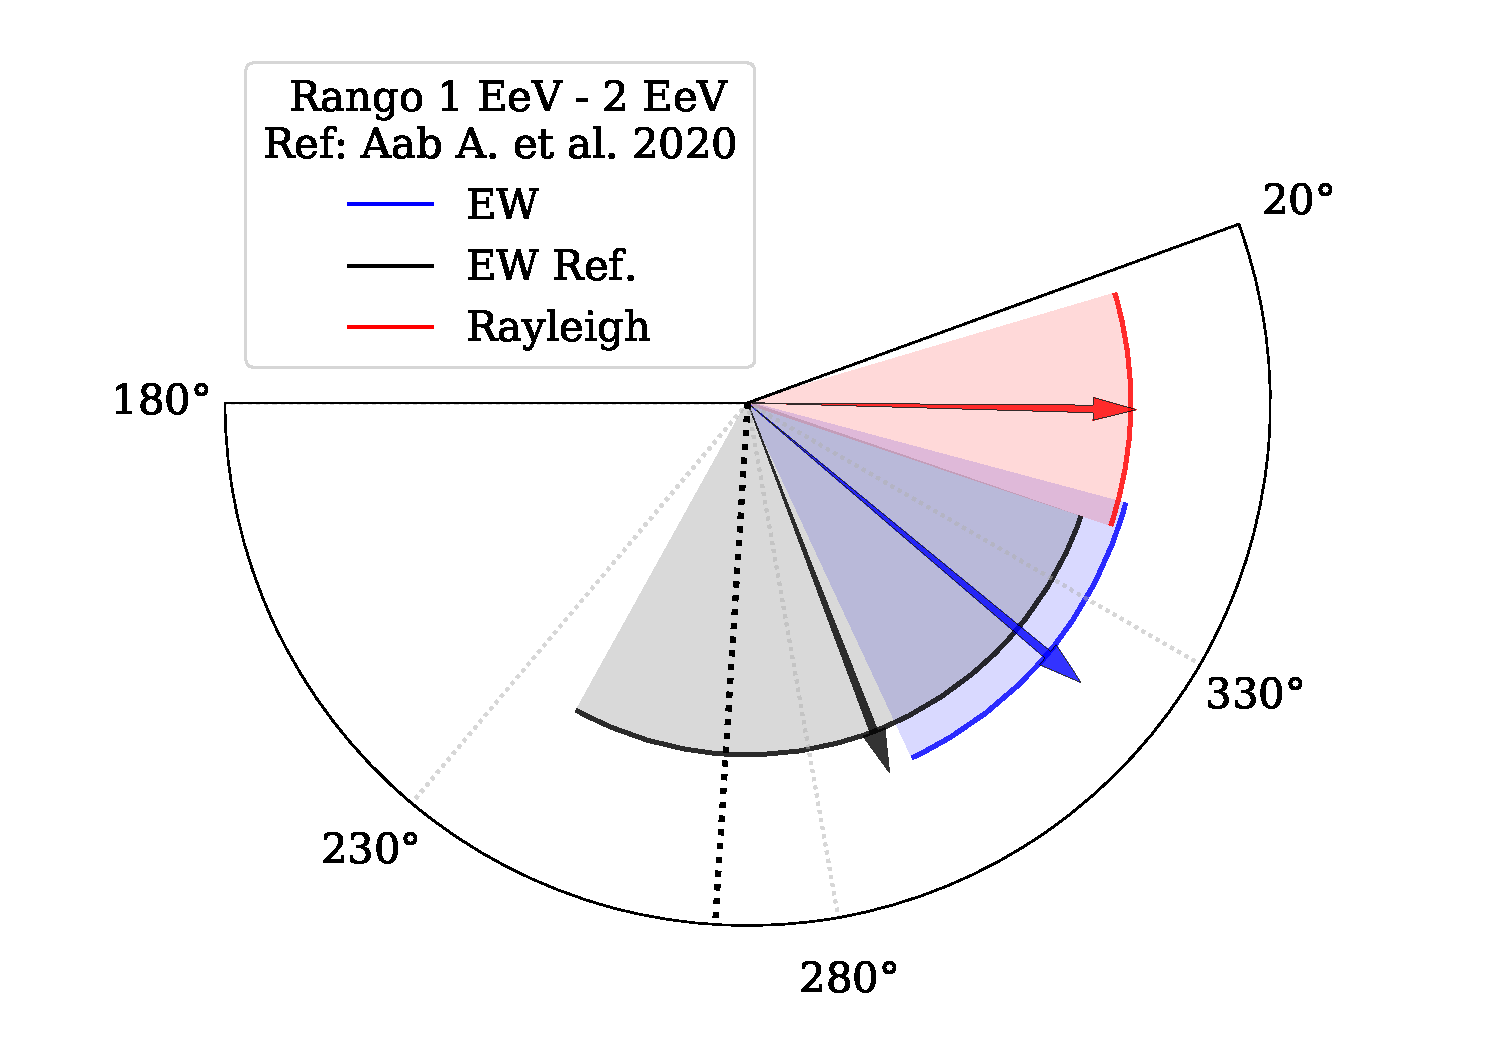
\includegraphics[width=0.75\textwidth]{phase_tercer_bin_v2.pdf}
            \end{center}
        \caption{Valores de las fases obtenidos en este trabajo y en la referencia con sus respectivas incertidumbres para la frecuencia sidérea en el  rango 1.0 EeV - 2.0 EeV .}
        \label{fig:tercer}
        \end{small}
    \end{figure}


    El barrido de frecuencias con la variable de la Ec.\ref{ra_arb} para este rango de energía se observa en la Fig.\ref{fig:tercer_barrido}. La línea horizontal indica el valor de $r_{99}$ para cada frecuencia y se observa que ninguna frecuencia supera dicho umbral. En la frecuencia solar no se observa ningún pico, esto se debe a que el método East - West es robusto con respecto a las modulación del clima. Se observa un pico en sidérea pero el mismo no es significativo con respecto al $r_{99}$.


    \begin{figure}[H]
        \begin{small}
            \begin{center}
                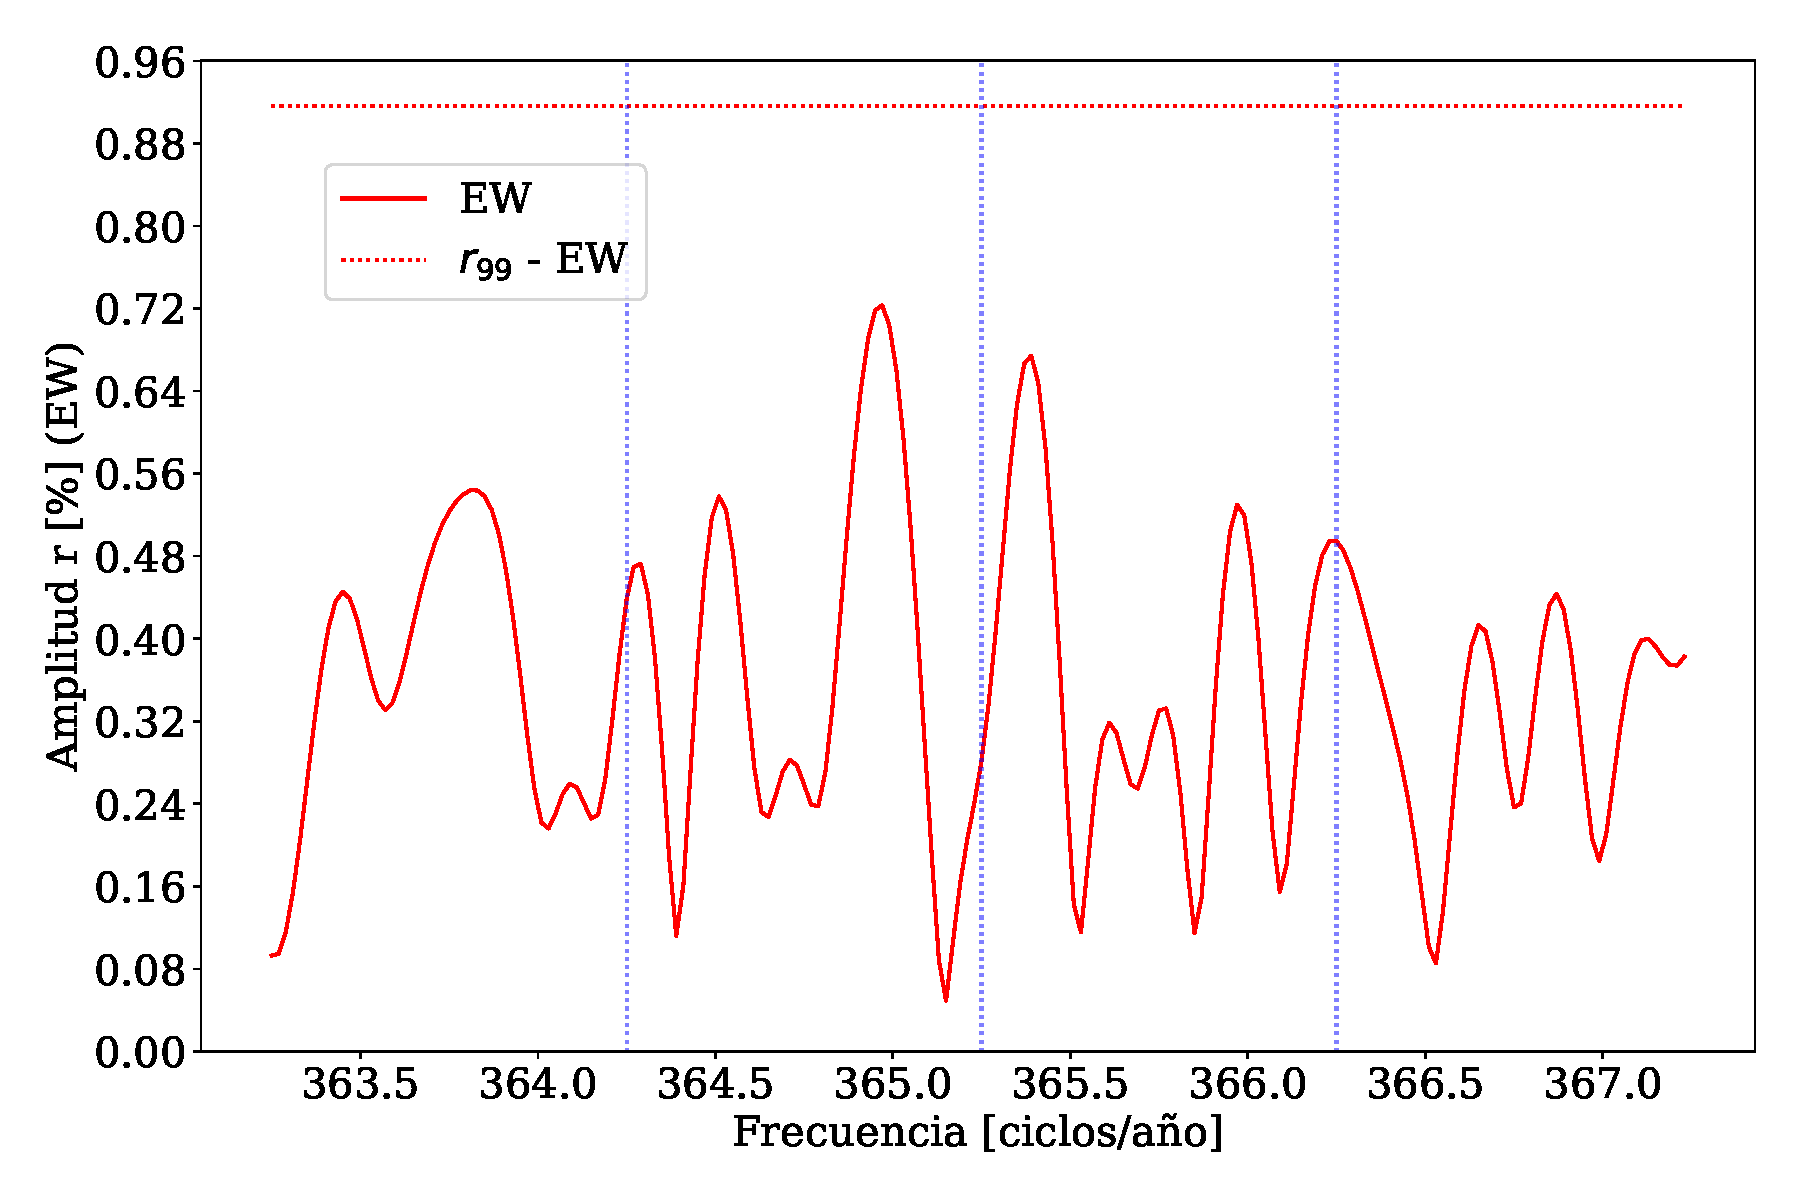
\includegraphics[width=0.75\textwidth]{plot_bin_3_barrido_v3_EW.pdf}
            \end{center}
            \caption{Barrido de frecuencias en el rango 1 EeV - 2 EeV .}
            \label{fig:tercer_barrido}
        \end{small}
    \end{figure}    

    \section{Gráficos}

    Para poder comparar los resultados de $d_\perp$ entre sí, podríamos graficar los valores de la proyección y de la límite del $99\%$ como se muestra en la Fig.\ref{fig:no_normalizado}. El inconveniente es la cantidad de datos en cada rango de energía entre los conjuntos de datos, todos los disparos y disparo estándar, son distintos.



    \begin{figure}[H]
        \begin{small}
            \begin{center}
                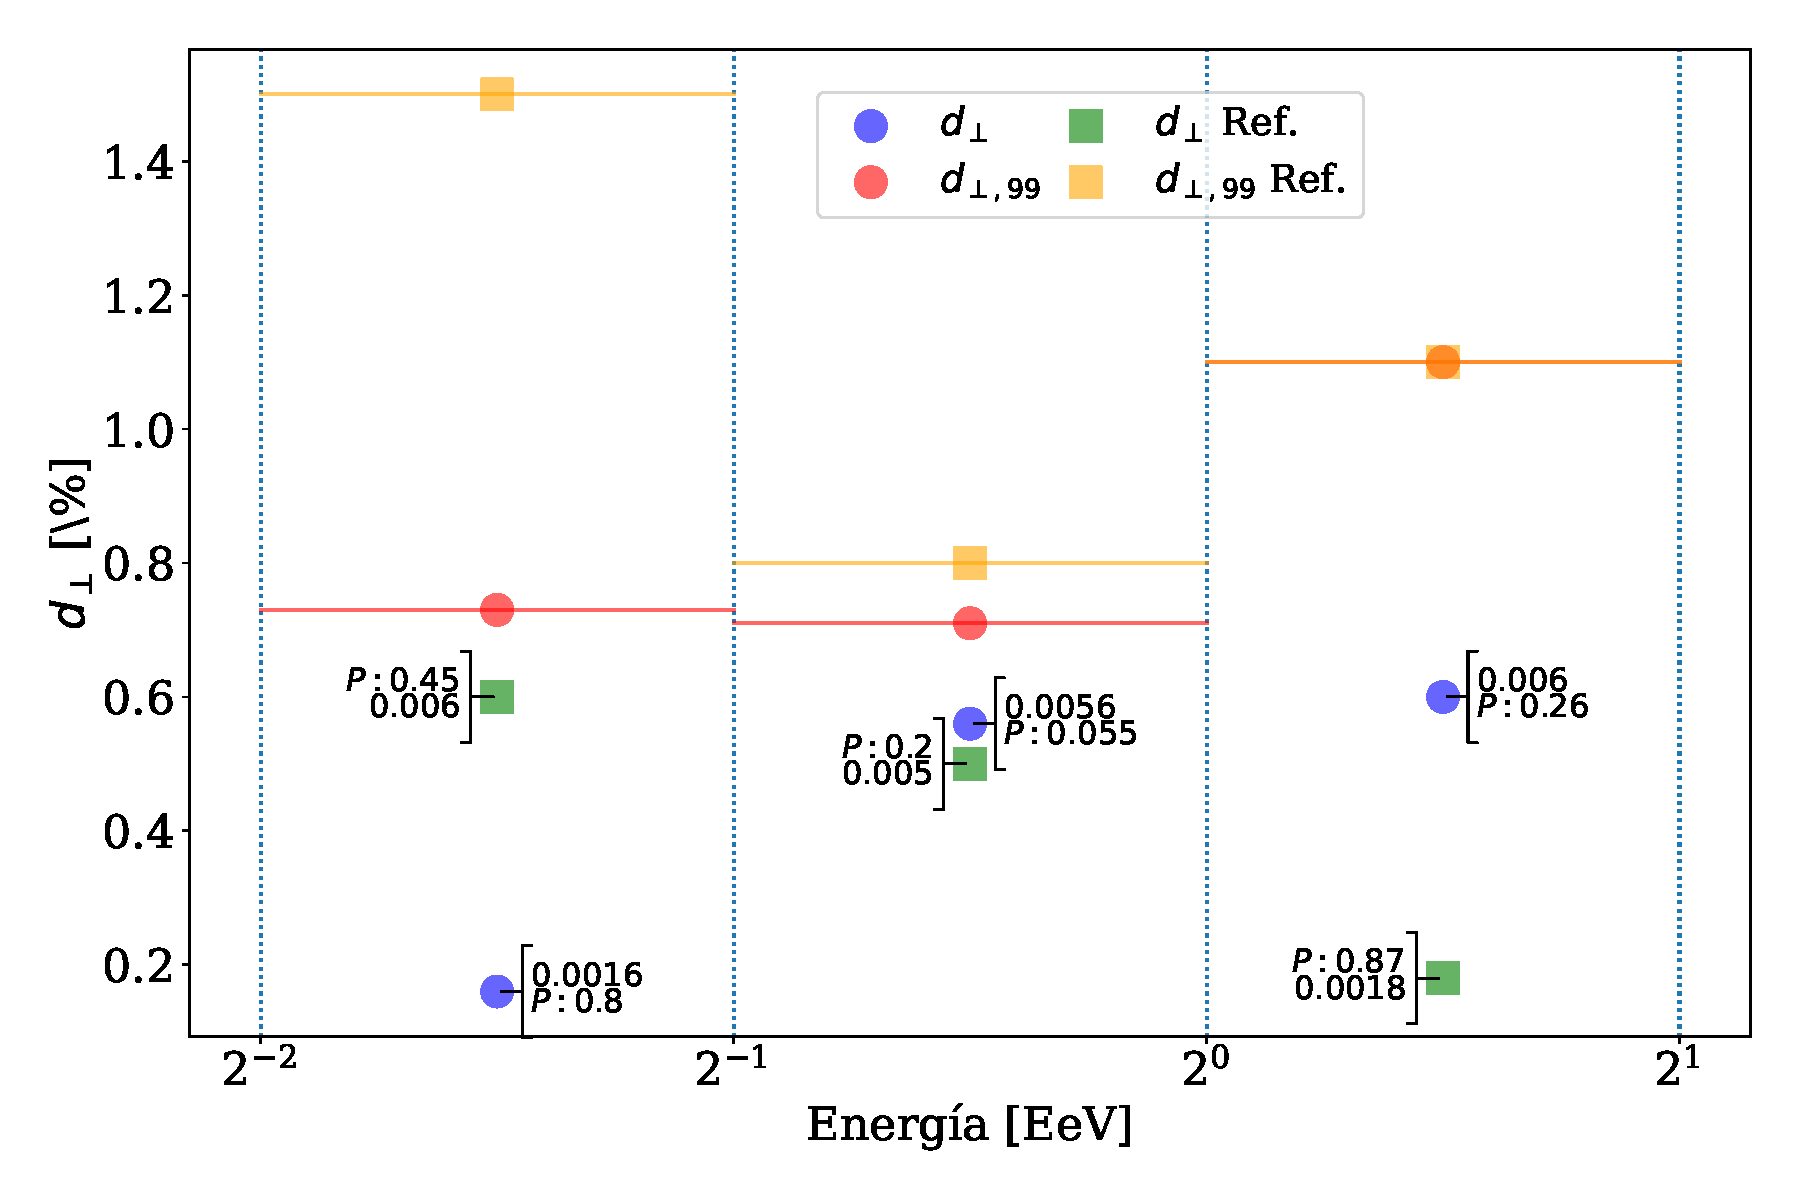
\includegraphics[width=0.75\textwidth]{d_perp_no_normalizado_v4.pdf}
            \end{center}
            \caption{Sin normalizar}
            \label{fig:no_normalizado}
        \end{small}
    \end{figure}
    
    % Para compararlos mejor con respecto a $d_{\perp,UL}$, usamos el valor de cada rango y de cada conjunto de datos, para normalizar la amplitud de $d_{\perp,UL}$. Como se muestra en la Fig.\ref{fig:normalizado}, ahora $d_{\perp,UL}=1$ y los otros valores se pueden comparar. 

    % \begin{figure}[H]
    %     \begin{small}
    %         \begin{center}
    %             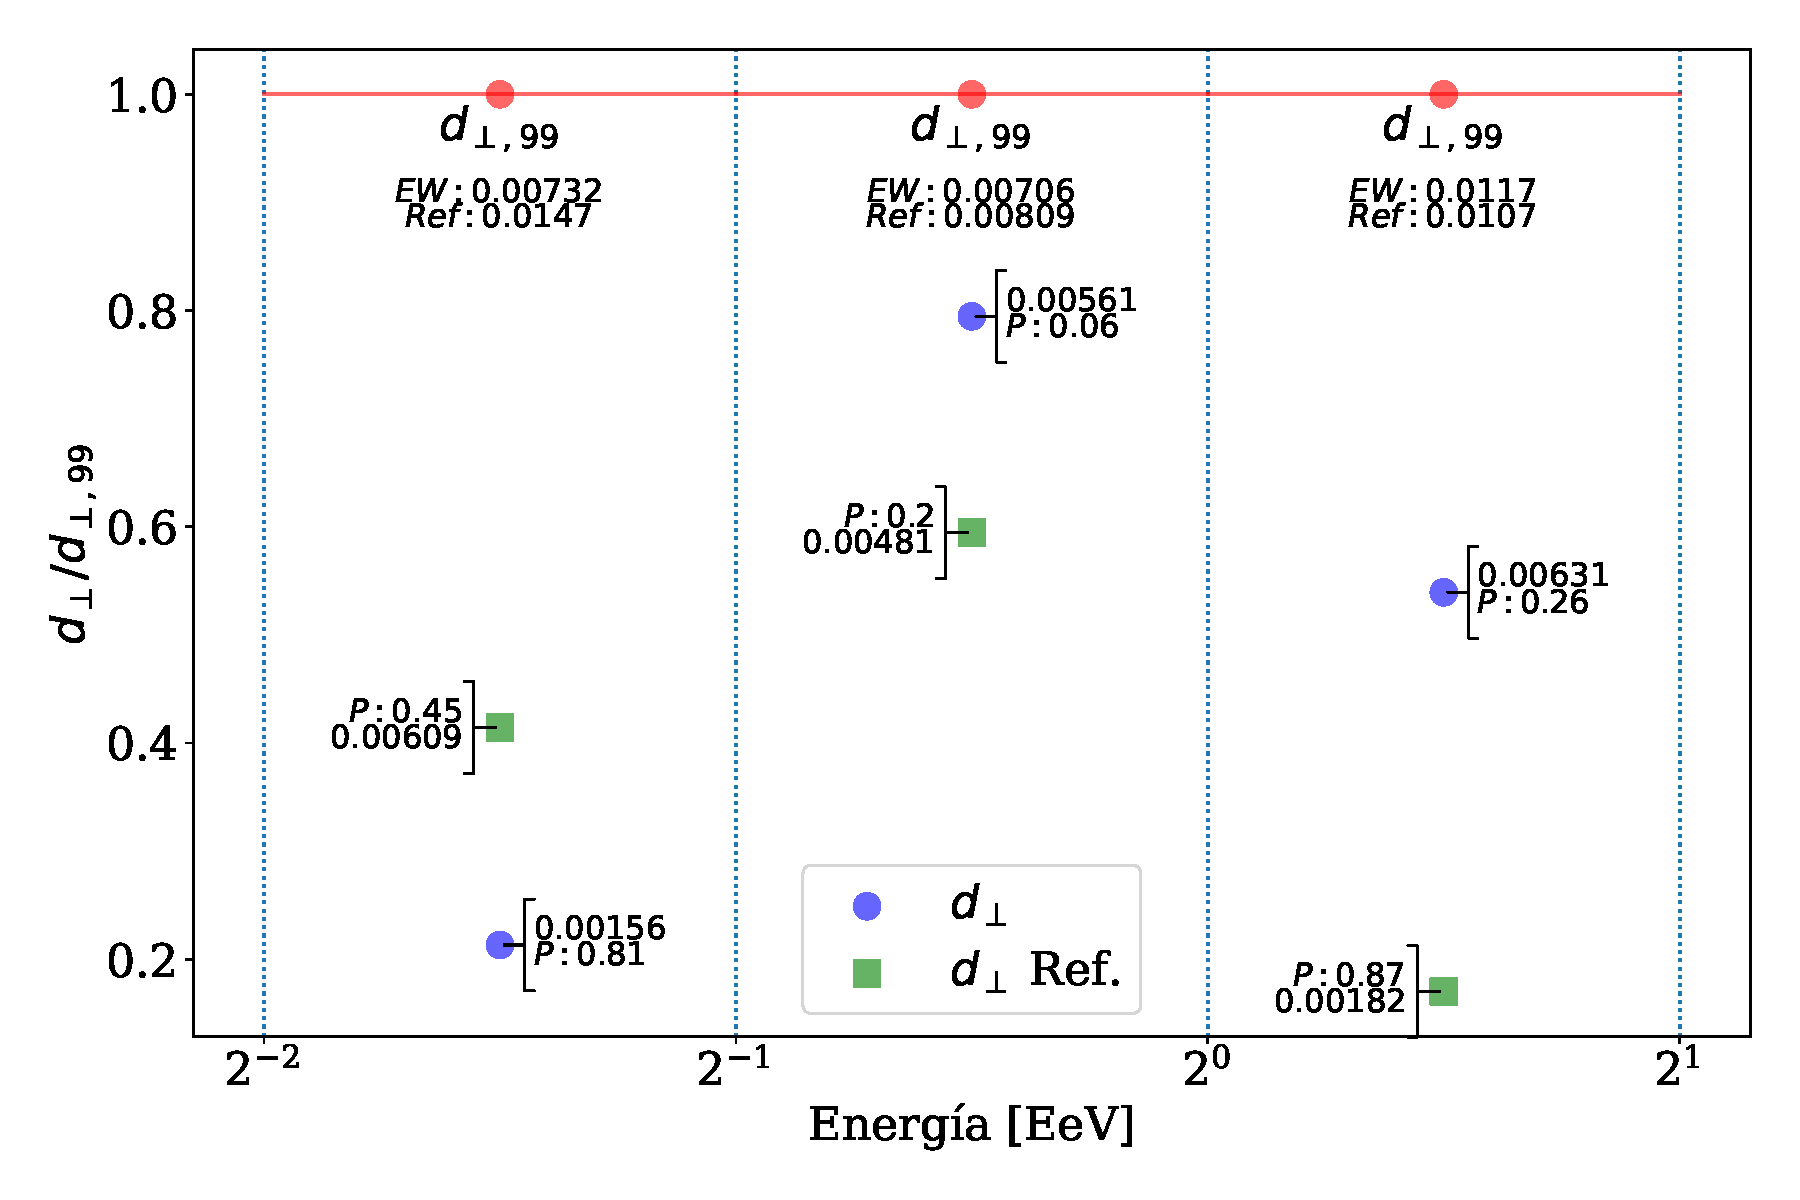
\includegraphics[width=0.75\textwidth]{d_perp_normalizado.pdf}
    %         \end{center}
    %         \caption{Valores normalizados con $d_{\perp,UL}$}
    %         \label{fig:normalizado}
    %     \end{small}
    % \end{figure}

    También podemos comparar cuan apartados están con respecto al valor $\sigma_{x,y}$ y normalizar los valores en cada rango de energía, así se obtiene la Fig.\ref{fig:normalizado_sigma}.

    \begin{figure}[H]
        \begin{small}
            \begin{center}
                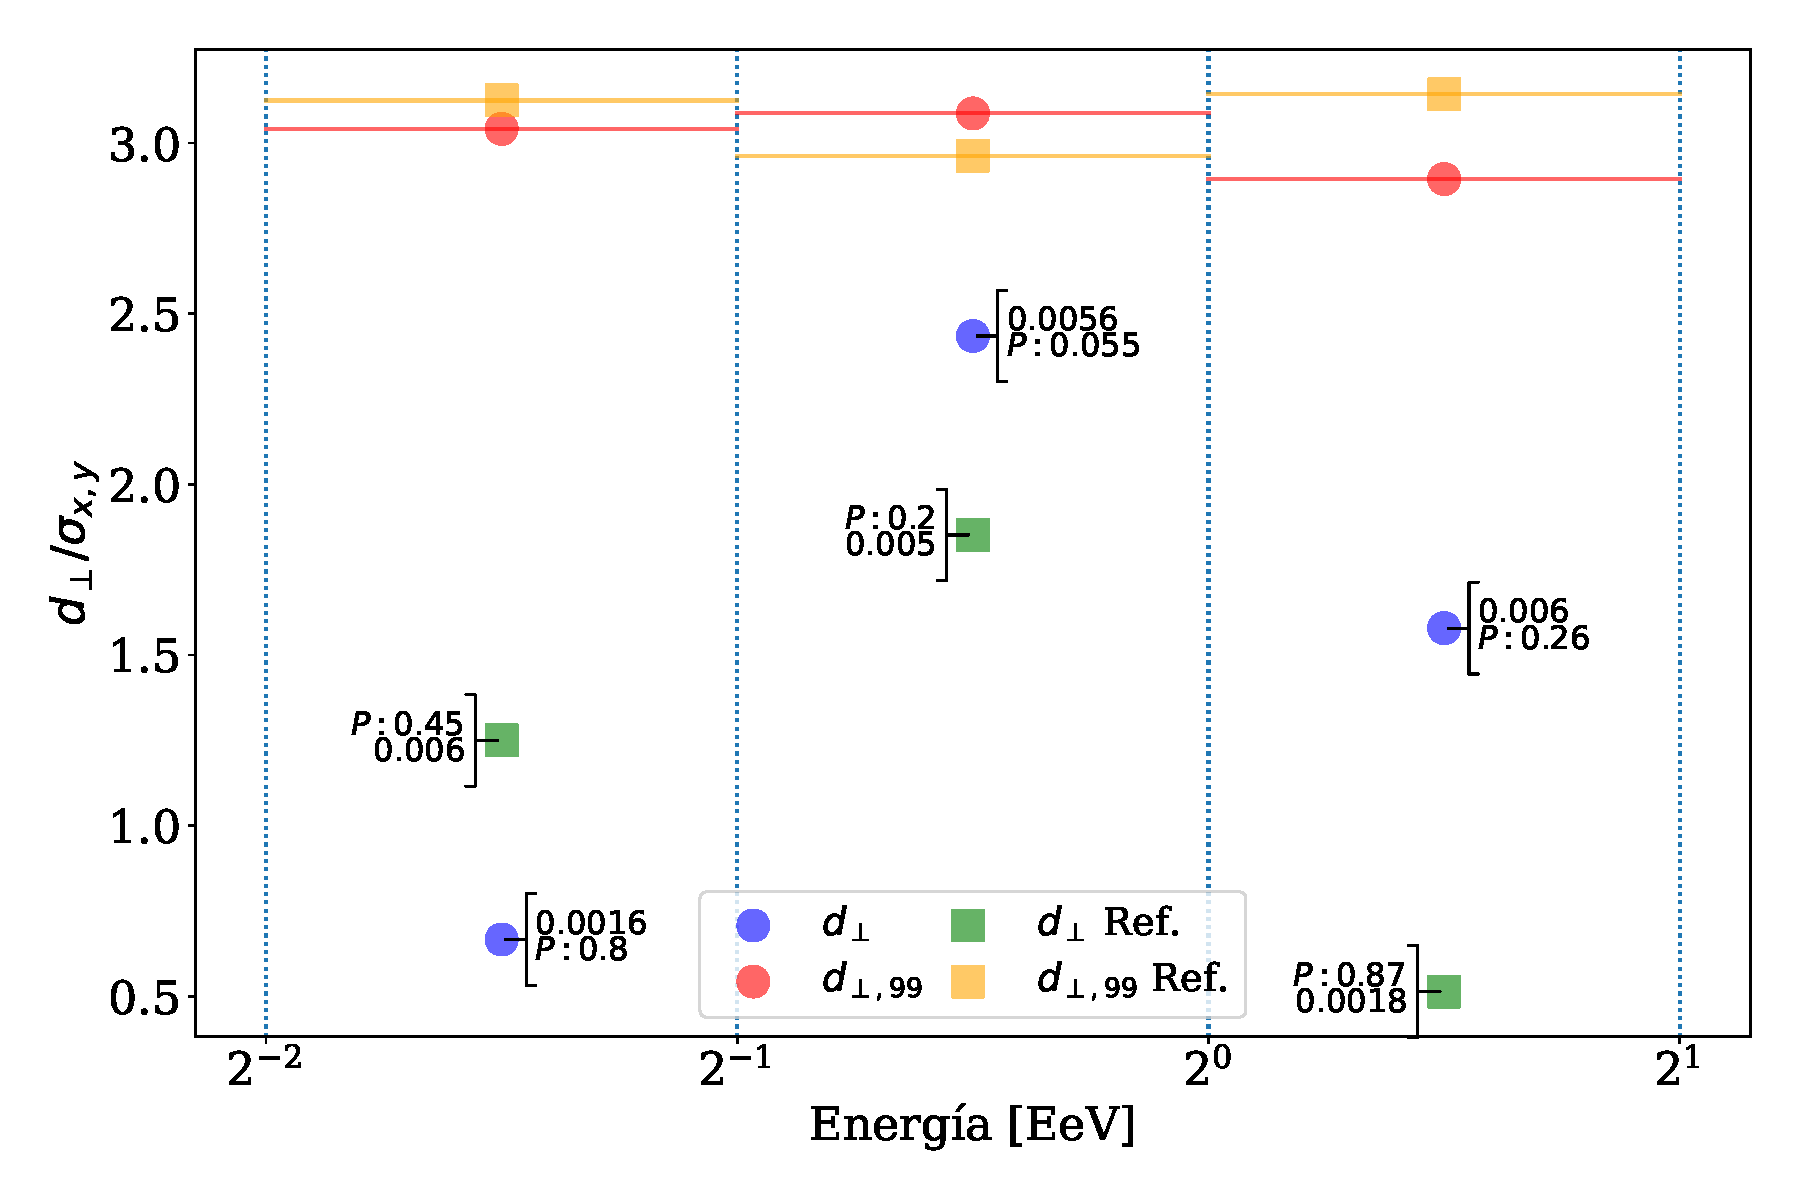
\includegraphics[width=0.75\textwidth]{d_perp_normalizado_sigmas_v5.pdf}
            \end{center}
            \caption{Valores normalizados con $d_{\perp,UL}$}
            \label{fig:normalizado_sigma}
        \end{small}
    \end{figure}

Por lo que ahora podemos decir que en los rangos entre 0.5 EeV - 1.0 EeV y 1.0 EeV - 2.0 EeV, la amplitud obtenida en este trabajo está por encima que la referencia. 

Para comparar los resultados en el  rango 0.25 EeV - 0.5 EeV, tenemos que tener en cuenta que el disparo estándar tiene una sensibilidad menor que el todos los disparos. Esto se ve claramente en la Tabla \ref{tab:}, donde el primer tiene 7 veces menos eventos para analizar. Por lo tanto, la discrepancia entre la referencia y los trabajos puede deberse a la  diferencia de eventos a estudiar causada por la sensibilidad del disparo.


Considerando los valores de $\sigma$ y $d_\perp$ para cada rango de energía, puedo comparar las direcciones, valores e incertidumbres en un sola figura como en la Fig.\ref{fig:incertidumbre}. Las líneas punteadas están centradas en los valores de referencia en cada rango de energía y con radio igual a sus incertidumbres. 

\begin{figure}[H]
    \begin{small}
        \begin{center}
            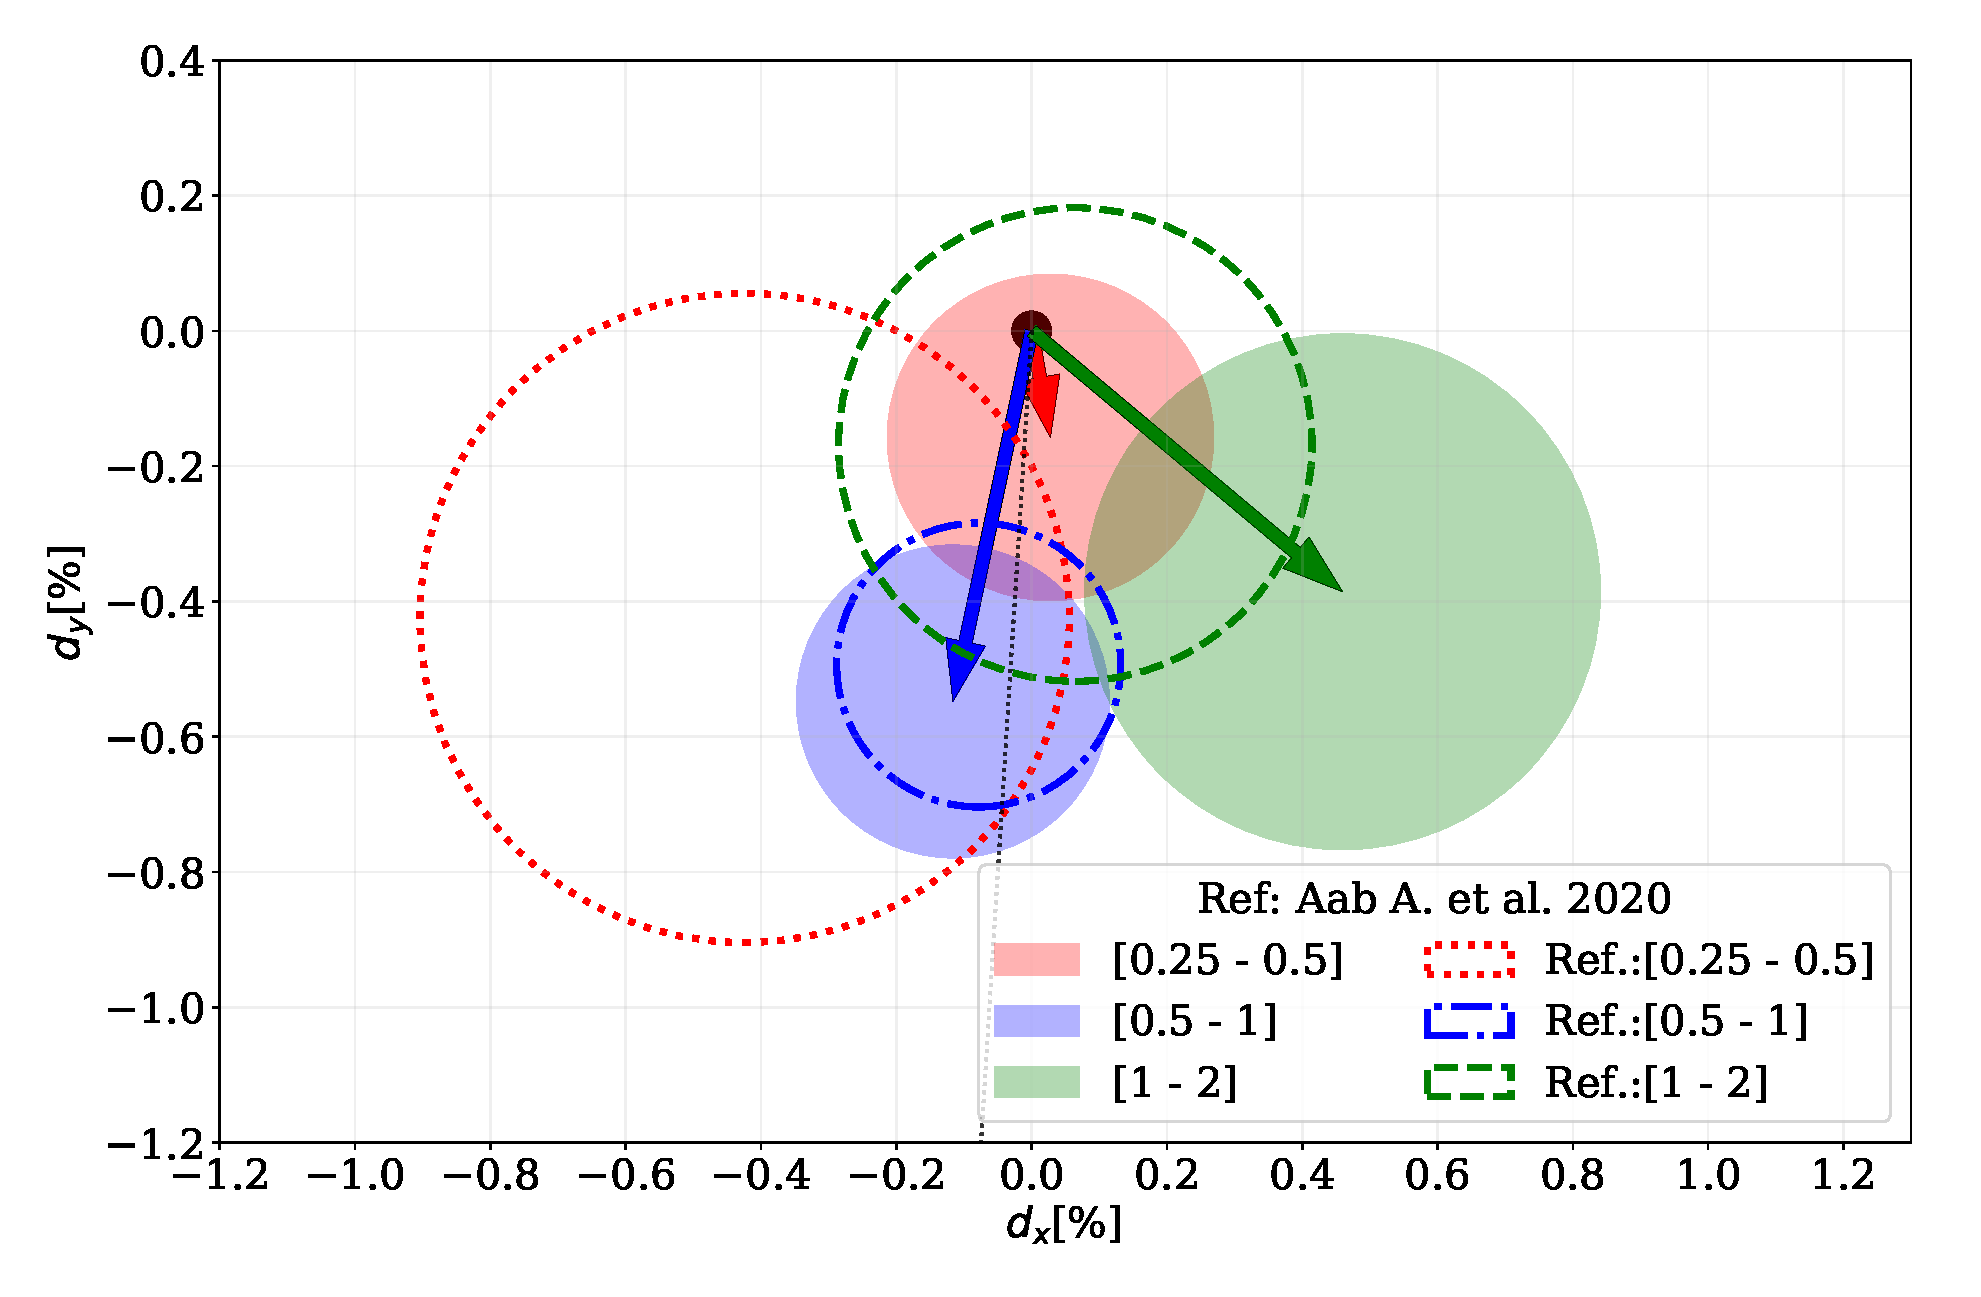
\includegraphics[width=0.9\textwidth]{comparando_sigmas_v3.pdf}
        \end{center}
        \caption{Amplitudes con incertidumbre, apuntando en la dirección  de la fase. Los círculos punteados los valores de referencia del trabajo \cite{Aab_2020} con sus respectivas incertidumbres y la línea punteada en negro marca la dirección del centro galáctico.}
        \label{fig:incertidumbre}
    \end{small}
\end{figure}


\chapter{Esto va a ir en otro capítulo que todavía no armé}
\section{Comparando resultados entre métodos para barridos de frecuencias}

\section{Verificación del código escrito durante la maestría}

Para ver que todo cierre, obtuve los resultados del paper \cite{Aab_2020} con el código del Rayleigh para distintos bines. En el bin  2 EeV - 4 EeV  tuve incongruencias entre mi código y los valores reportados en el paper, pero si comparo los valores obtenidos con el código utilizado para el paper con mis resultados si se corresponden. En los demás bines los resultados entre el código implementado en \cite{Aab_2020}, los resultados publicados y los resultados de mi código se corresponden.


En el bin 2 EeV - 4 EeV, verifiqué sin cambiaba los números considerando los eventos hasta $80^o$, pero los parámetros de Rayleigh eran los mismos que usar $60^o$  como límite en $\theta$.  Cuando no considero los pesos en mi código, obtengo resultados congruentes con los publicados pero eso puedo ser una casualidad.

\begin{table}[H]
    \begin{small}
        \begin{center}
            \begin{tabular}[c]{l|c|c|c|c|}
                                            & \multicolumn{4}{|c|}{2 EeV - 4 EeV}                                                               \\ \hline
                Frecuencia:                 & Sidérea              & Sidérea (Sin pesos)  & Sidérea \cite{codigo}    & Sidérea \cite{Aab_2020}   \\ \hline
                Amplitud r [\%]:            & $0.5^{+0.3}_{-0.2}$ & $0.4^{+0.3}_{-0.2}$ & $0.5^{+0.3}_{-0.2}$     & -                          \\
                $r_{99}$ [\%]:              & 0.8                 & 0.8                 & 0.8                     & -                          \\\hline
                Amplitud $d_\perp$[\%]:     & $0.7^{+0.4}_{-0.2}$ & $0.5^{+0.4}_{-0.2}$ & $0.7^{+0.4}_{-0.2}$ 	  & $0.5^{+0.4}_{-0.2}$                    \\
                $d_{99}$ [\%]:              & 1.0                 & 1.0                 & 1.0                     & -                         \\
                $d_{\perp,UL}$[\%]:         & 1.9                 & 1.7                 & -                       & 1.4                               \\\hline
                $\sigma_{x,y}$[\%]:         & 0.34	              & 0.34	            & 0.34	                  & 0.34                           \\
                Probabilidad      :         & 0.14                & 0.33                & 0.15               	  & 0.34                       \\
                Fase[$^o$]:                 & 355$\pm$29          & 351$\pm$38          & 346$\pm$29              & 349$\pm$55                    \\\hline
            \end{tabular}
        \end{center}
    \end{small}
    \caption{Características para las frecuencias solar y sidérea con el método Rayleigh en el primer armónico en el rango de energía 2 EeV - 4 EeV, obtenidos con el código de este trabajo aplicado al conjunto de datos de la referencia \cite{Aab_2020} y comparados con los resultados reportados en el último.}
\end{table}


\begin{table}[H]
    \begin{small}
        \begin{center}
            \begin{tabular}[c]{l|c|c||c|c|}
                                            & \multicolumn{2}{c||}{8 EeV - 16 EeV}              & \multicolumn{2}{c|}{16 EeV - 32 EeV}                   \\ \hline
                Frecuencia:                 & Sidérea                    & Sidérea \cite{Aab_2020} & Sidérea                   & Sidérea \cite{Aab_2020}   \\ \hline
                Amplitud r [\%]:            & $4.4^{+1.0}_{-0.8}$ 	    & -                      & $5.8^{+1.8}_{-1.3}$ 	    & -                         \\
                $r_{99}$ [\%]:              & 2.6                       & -                      & 4.9                      & -                          \\\hline
                Amplitud $d_\perp$[\%]:     & $5.6^{+1.2}_{-1.0}$ 	    & $5.6^{+1.2}_{-1.0}$    & $7.5^{+2.3}_{-1.8}$ 	    & $7.5^{+2.3}_{-1.8}$                   \\
                $d_{99}$ [\%]:              & 3.3                       & -                      & 6.3                      & -                         \\
                $d_{\perp,UL}$[\%]:         & 10                        & -                      & 16                       & -                                 \\\hline
                $\sigma_{x,y}$[\%]:         & 1.1	                    & 1.1                    & 2.1	                    & 2.1                           \\
                Probabilidad      :         & $2.3\times10^{-6}$	    & $2.3\times10^{-6}$     & $1.5\times10^{-3}$	    & $1.5\times10^{-3}$              \\
                Fase[$^o$]:                 & 96$\pm$11                 & 97$\pm$12              & 80$\pm$16                & 80$\pm$17                     \\\hline
            \end{tabular}
        \end{center}
    \end{small}
    \caption{Características para las frecuencias solar y sidérea con el método Rayleigh en el primer armónico en distintos rangos de energía, obtenidos con el código de este trabajo aplicado al conjunto de datos de la referencia \cite{Aab_2020} y comparados con los resultados reportados en el último.}
\end{table}


\section{Comparando amplitud en función de la frecuencia}

En las Figs.\ref{fig:primer_barrido_EW_Ray}, \ref{fig:segundo_barrido_EW_Ray} y \ref{fig:tercer_barrido_EW_Ray} se comparan el barrido en frecuencia con el método East - West y el barrido con Rayleigh considerando los pesos de los hexágonos en distintos rangos de energía.


\begin{figure}[H]
    \begin{small}
        \begin{center}
            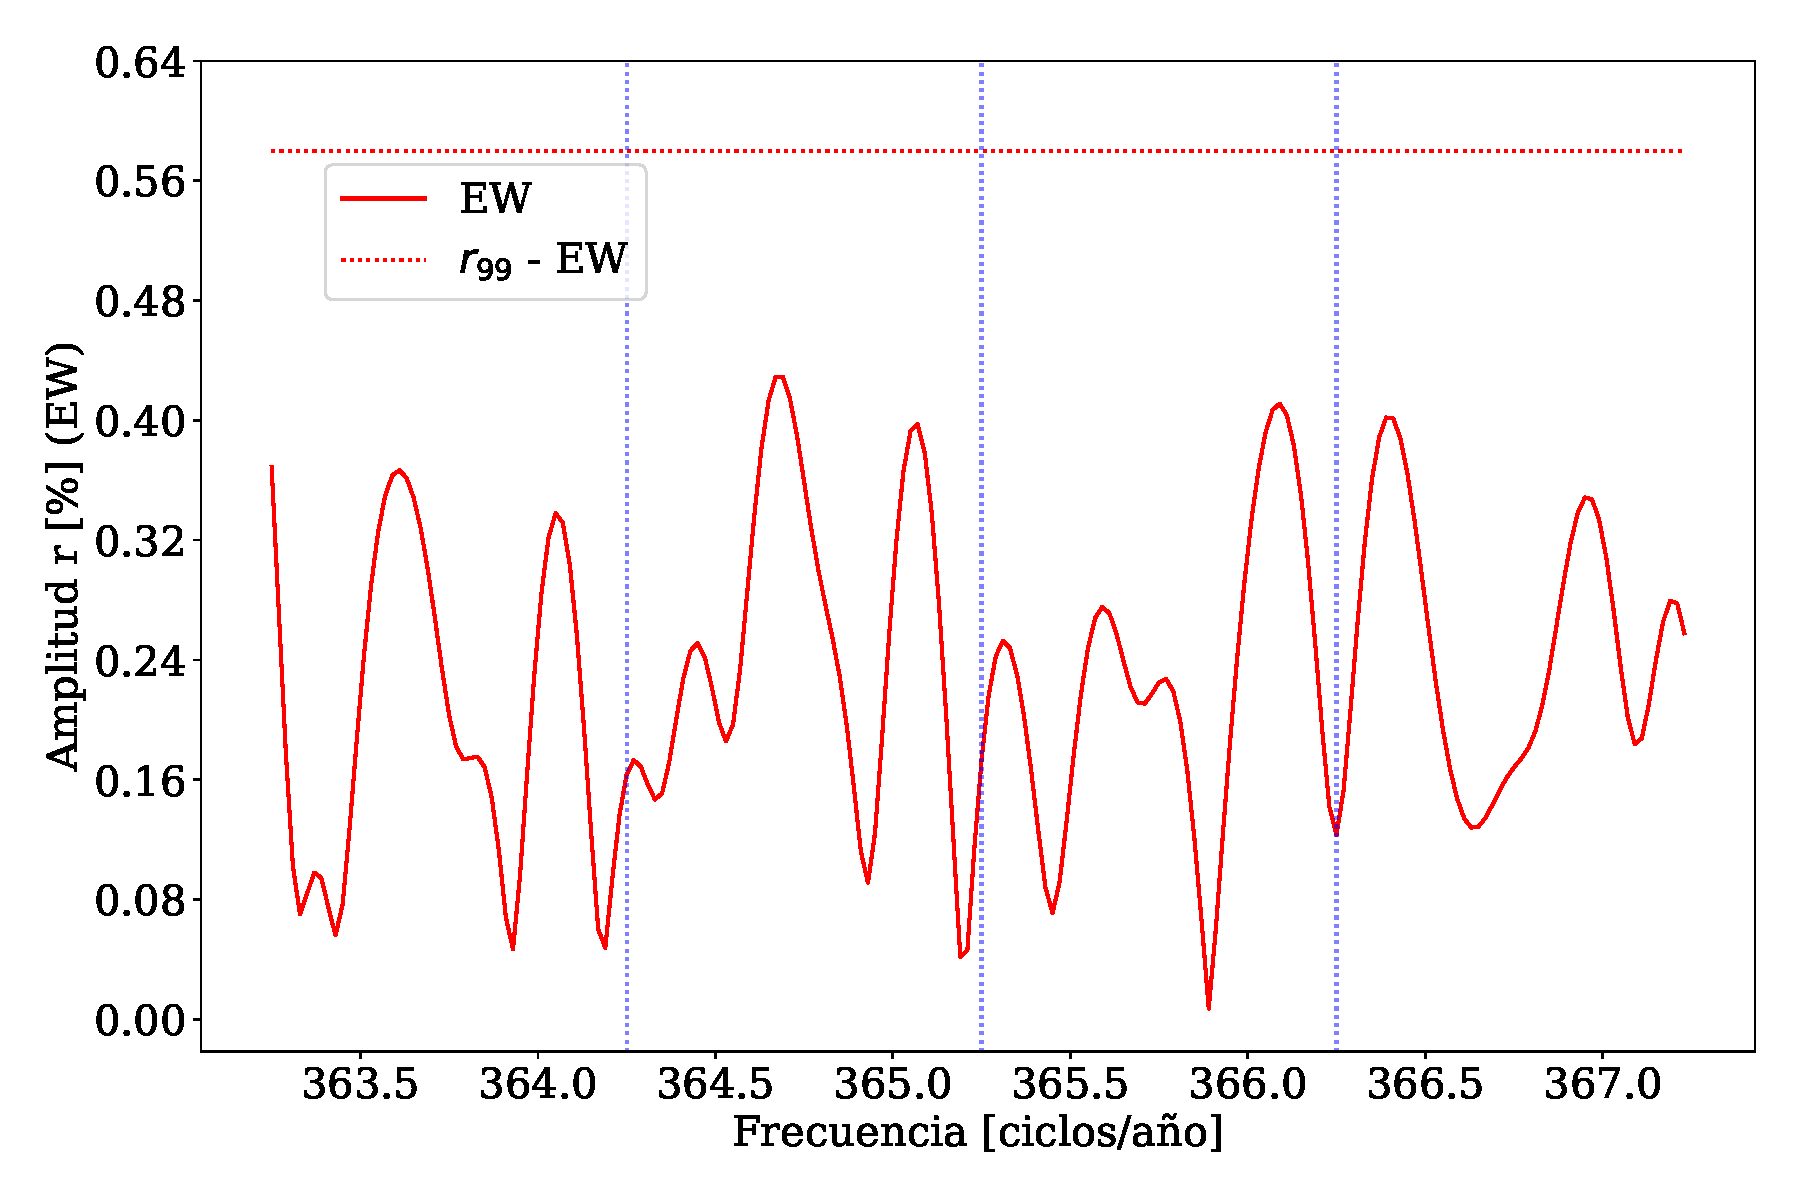
\includegraphics[width=0.4955\textwidth]{plot_bin_1_barrido_v3_EW.pdf}
            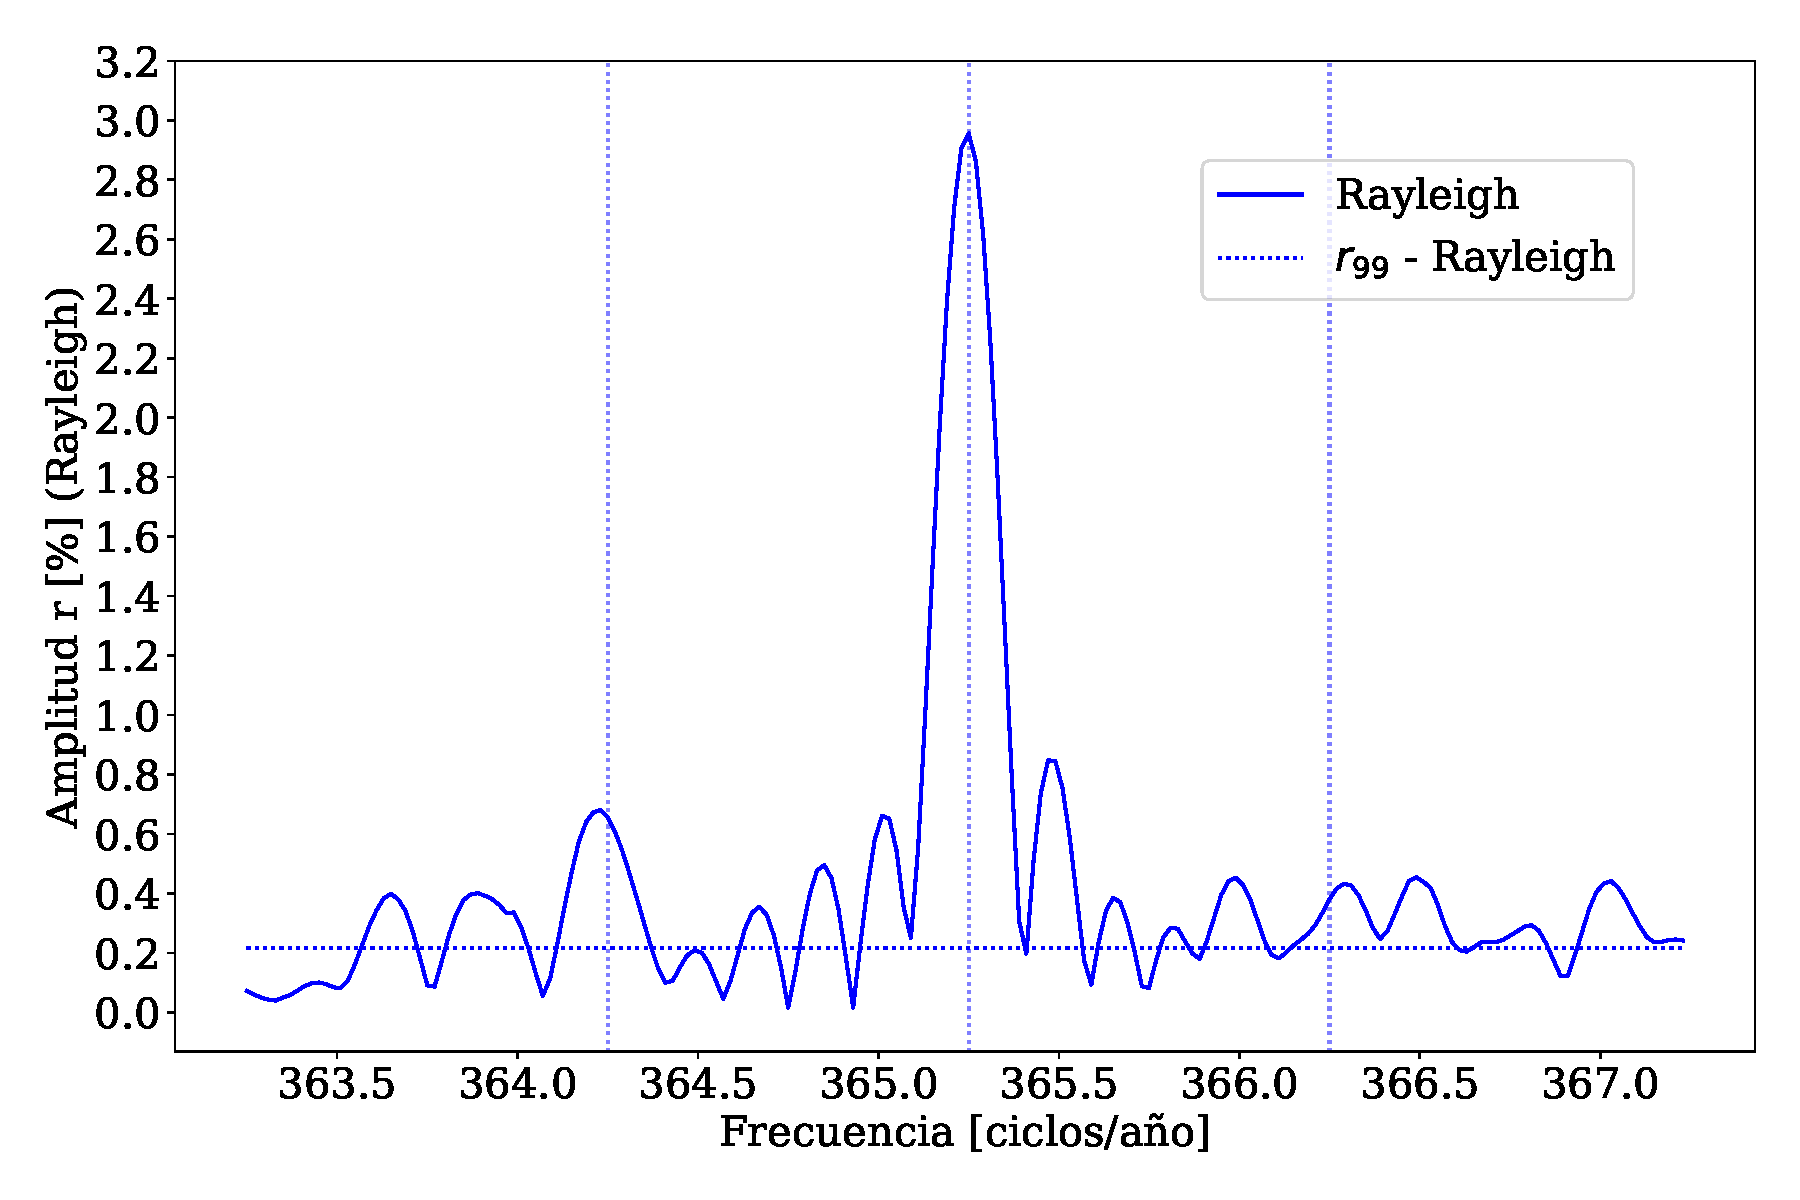
\includegraphics[width=0.4955\textwidth]{plot_bin_1_barrido_v1_Ray.pdf}
        \end{center}
        \caption{Barrido de frecuencias en el rango 0.25 EeV - 0.5 EeV .}
        \label{fig:primer_barrido_EW_Ray}
    \end{small}
\end{figure}    

\begin{figure}[H]
    \begin{small}
        \begin{center}
            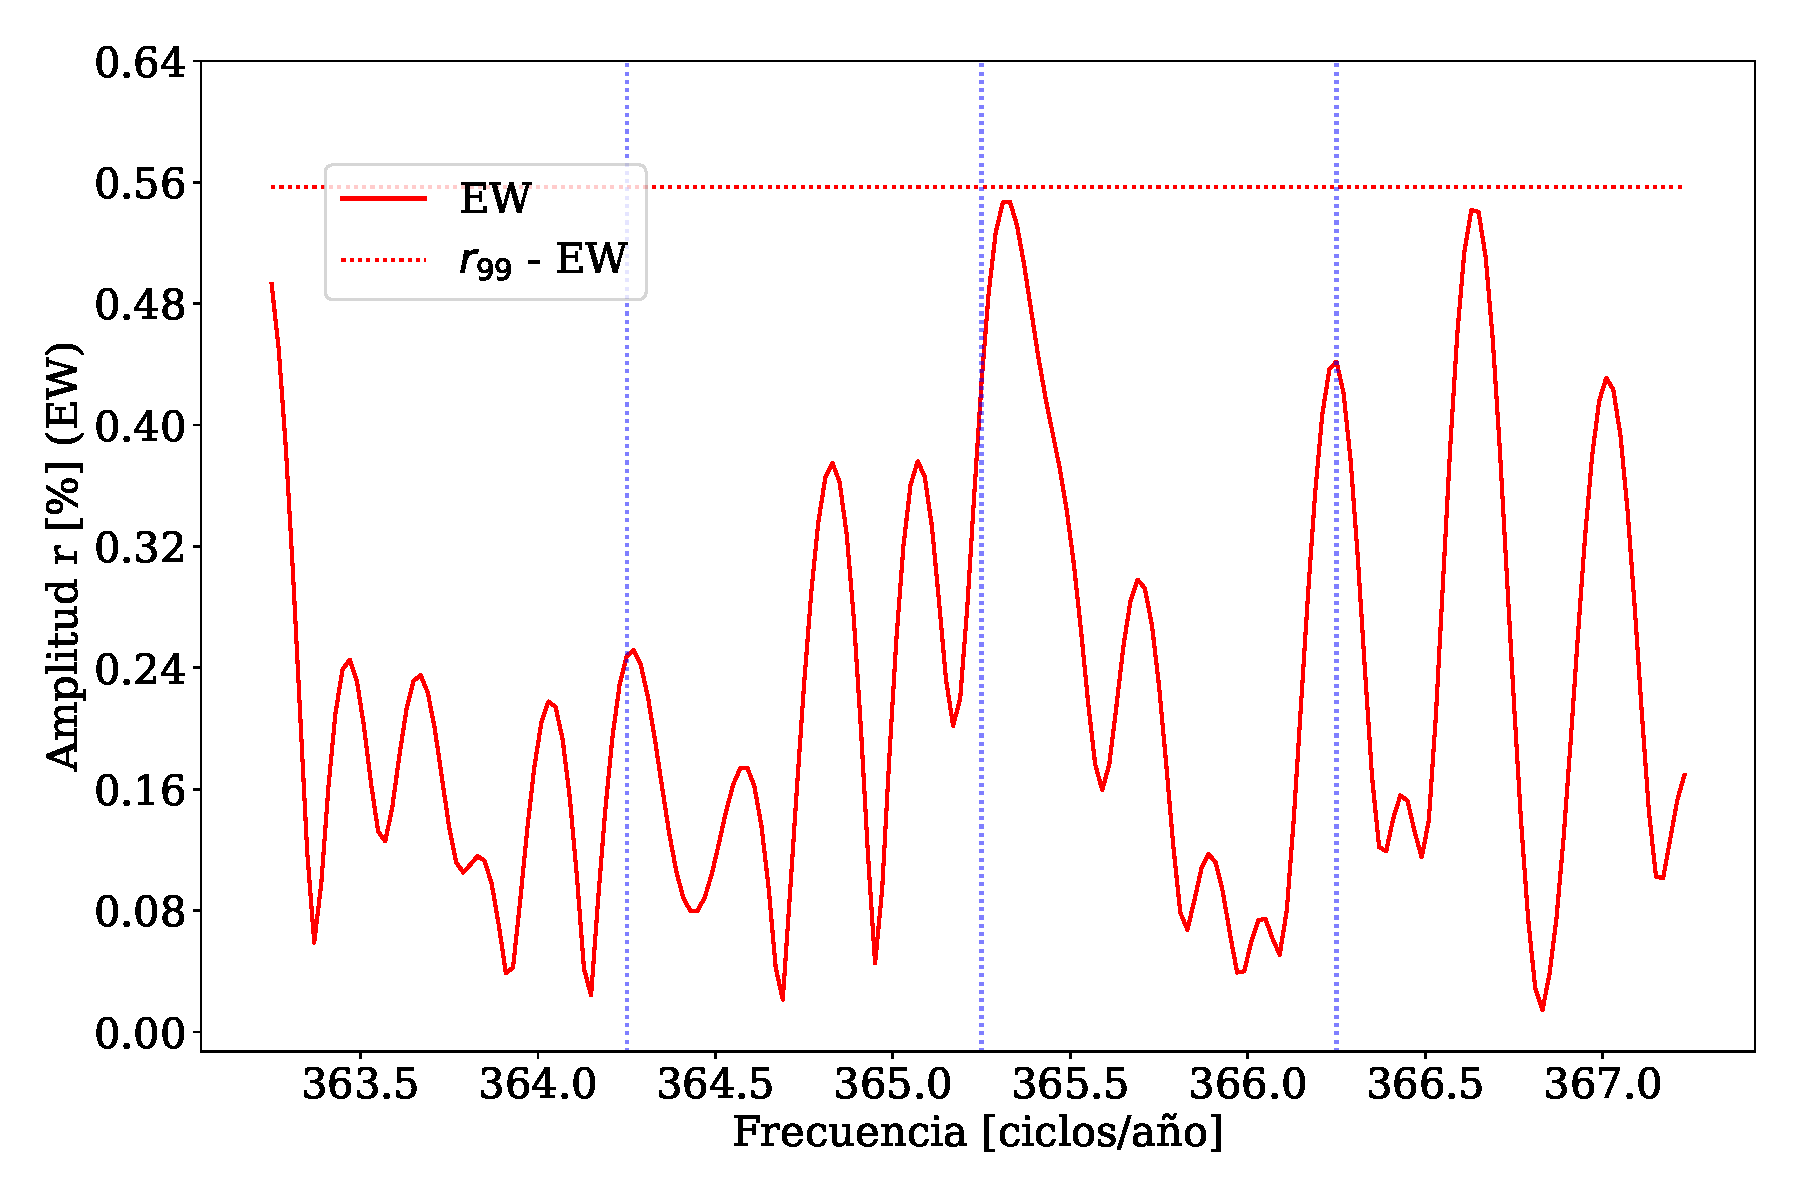
\includegraphics[width=0.4955\textwidth]{plot_bin_2_barrido_v3_EW.pdf}
            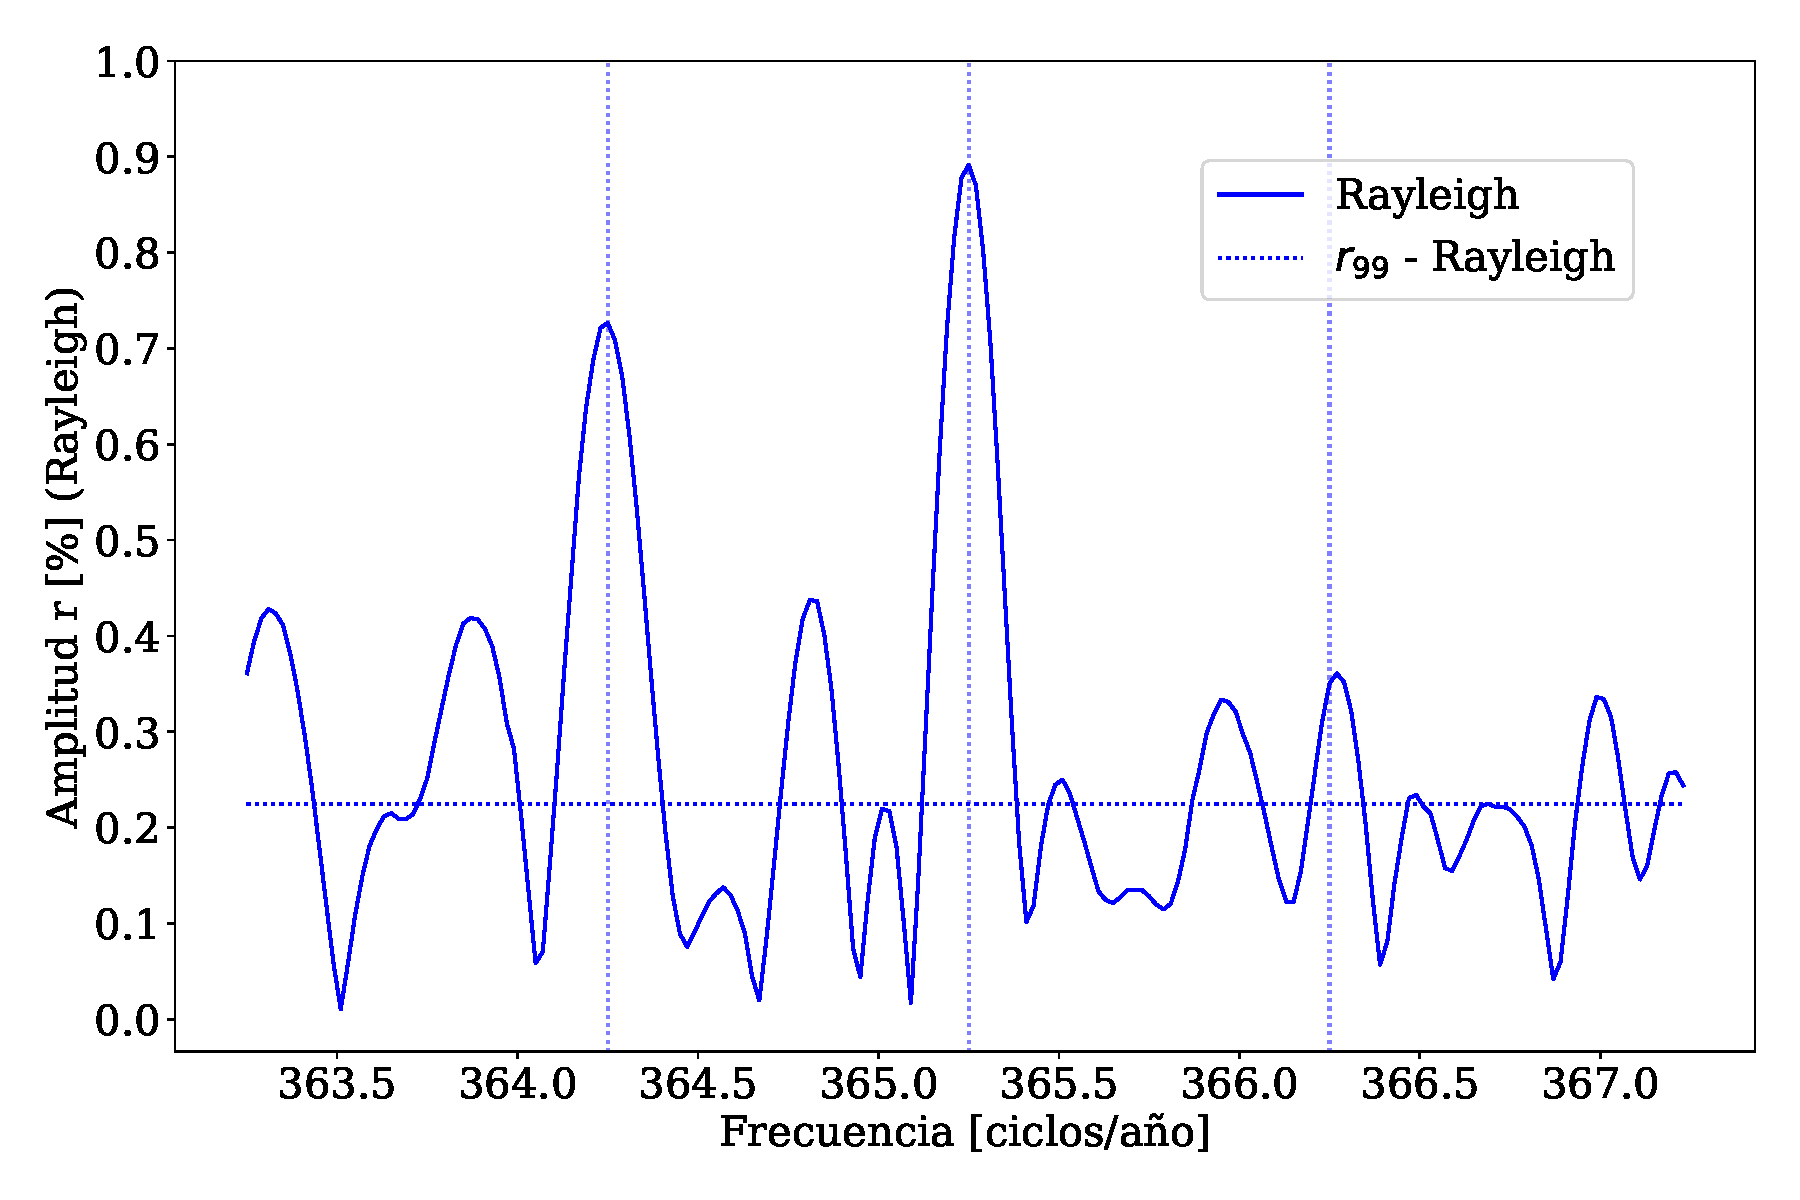
\includegraphics[width=0.4955\textwidth]{plot_bin_2_barrido_v1_Ray.pdf}
        \end{center}
        \caption{Barrido de frecuencias en el rango 0.5 EeV - 1 EeV .}
        \label{fig:segundo_barrido_EW_Ray}
    \end{small}
\end{figure}    

\begin{figure}[H]
    \begin{small}
        \begin{center}
            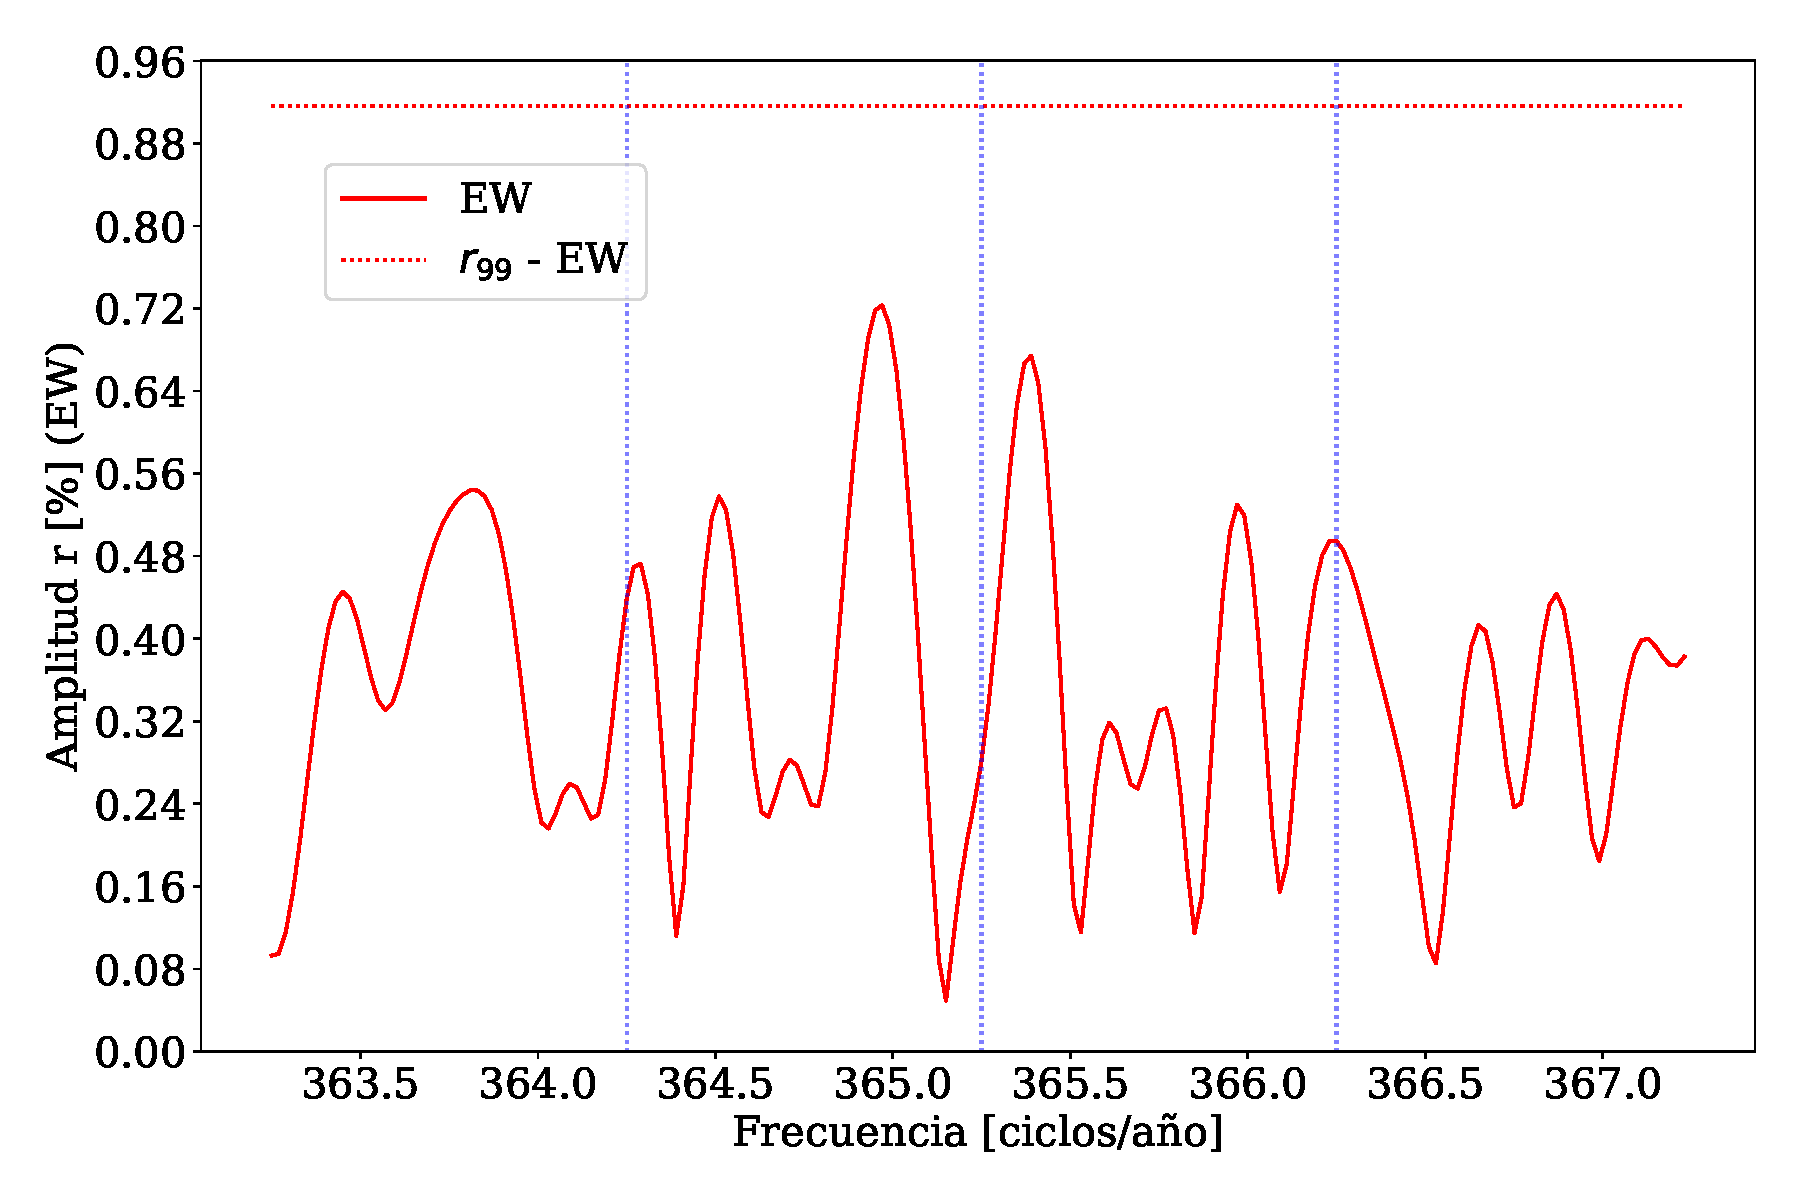
\includegraphics[width=0.4955\textwidth]{plot_bin_3_barrido_v3_EW.pdf}
            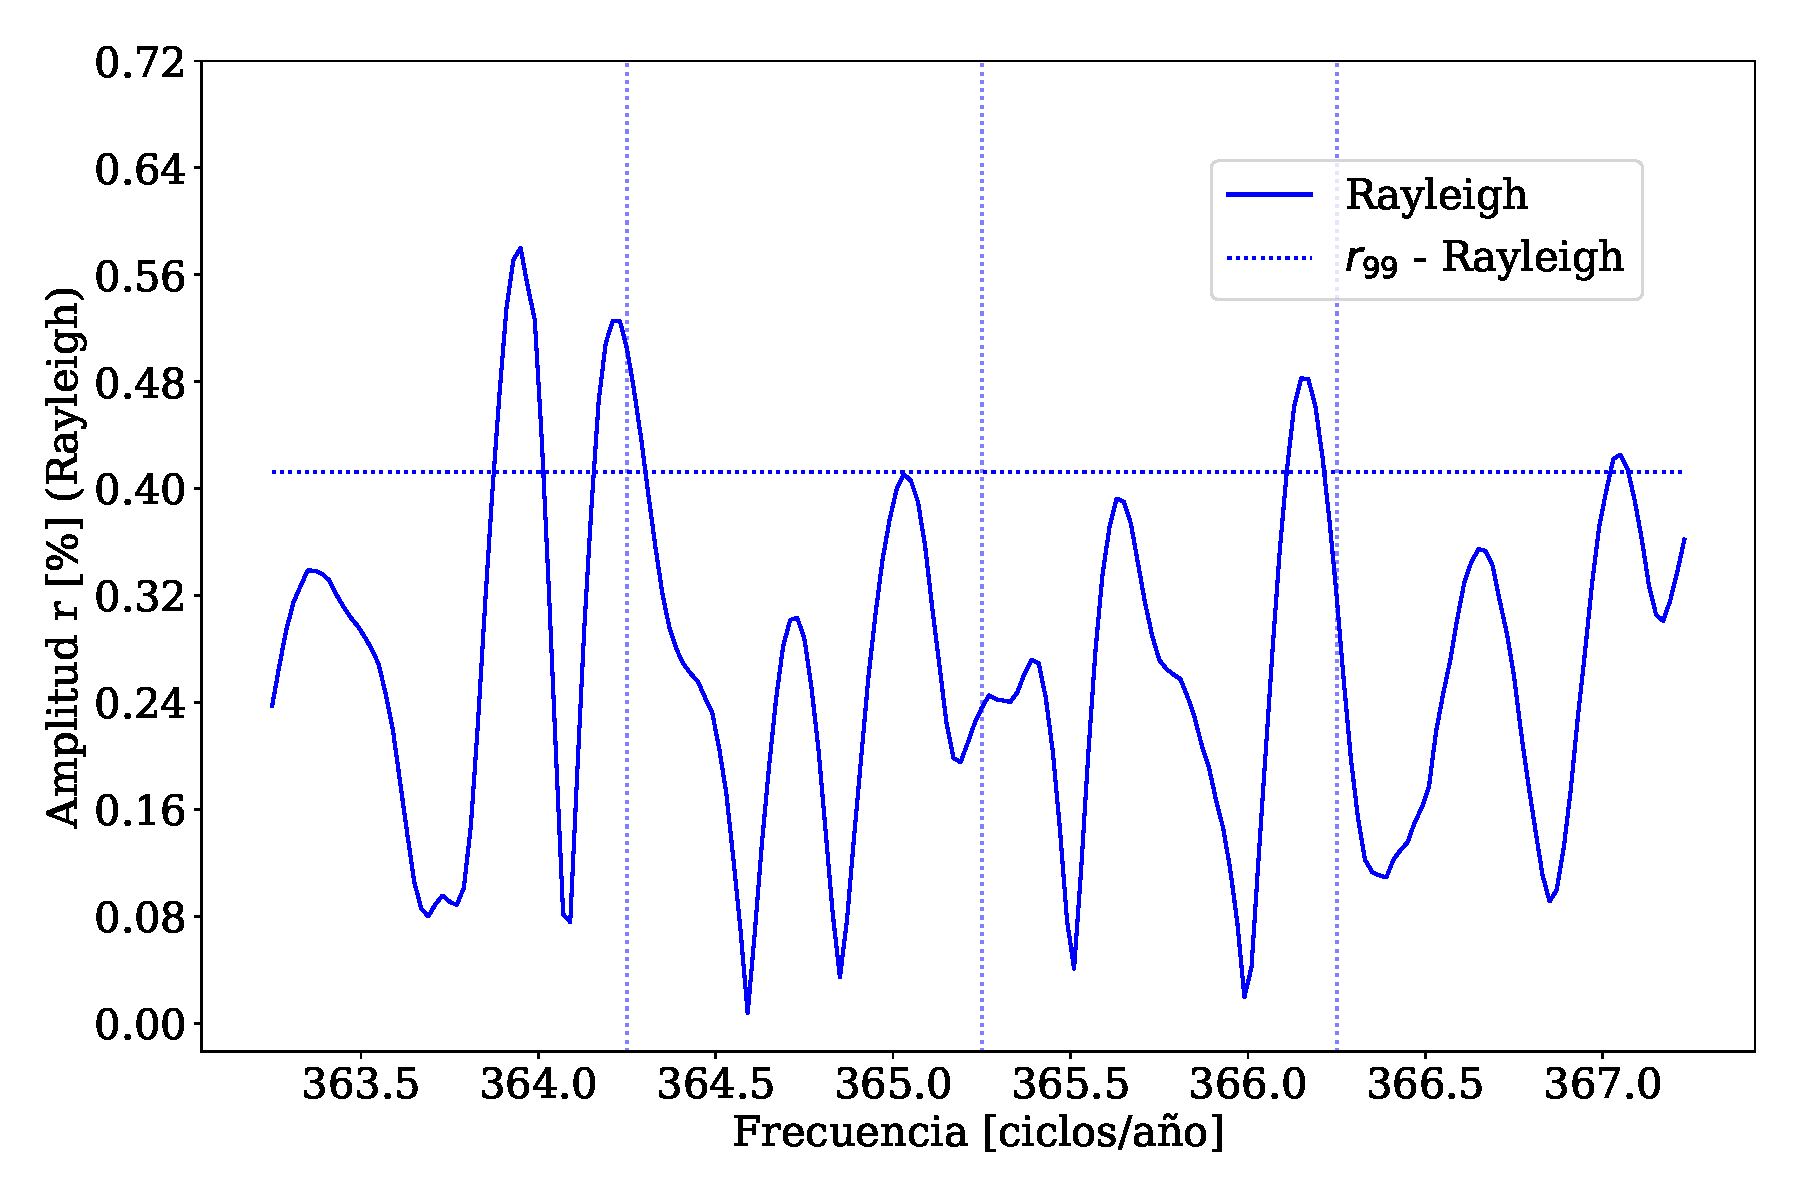
\includegraphics[width=0.4955\textwidth]{plot_bin_3_barrido_v1_Ray.pdf}
        \end{center}
        \caption{Barrido de frecuencias en el rango 1 EeV - 2 EeV .}
        \label{fig:tercer_barrido_EW_Ray}
    \end{small}
\end{figure}    



\begin{biblio}
	\bibliography{mibib_16.bib, ../Tesis/mibib.bib}
\end{biblio}
    
    \end{document}
